%\documentclass{frontiersENG} % for Engineering articles
\documentclass{frontiersSCNS} % for Science articles
%\documentclass{frontiersMED} % for Medicine articles
%\documentclass{frontiersFPHY} % for Physics articles


%\usepackage[utf8x]{inputenc}
%\usepackage[T1]{fontenc}

%\usepackage[english]{babel}

\usepackage{graphicx}
\graphicspath{{figs/}}
\usepackage{tikz}
\usetikzlibrary{shapes}
\usetikzlibrary{svg.path}
%
\usepackage{amsmath} 
\usepackage{mathptmx}      % use Times fonts if available on your TeX system
%
\usepackage{color, soul}
\usepackage{url}
\usepackage{multirow}
\usepackage{array}
\usepackage{fixltx2e}
\usepackage{textcomp}

\usepackage{caption}
\usepackage{subcaption}
\usepackage{float}
\floatstyle{plaintop}

\usepackage{paralist} % inparaenum

\usepackage[bookmarks]{hyperref}

\usepackage[draft, nomargin, marginclue, footnote]{fixme}
\fxsetup{targetlayout=color}

\newcommand{\eg}{{\textit{e.g.~}}}
\newcommand{\etal}{{\textit{et al.~}}}
\newcommand{\ie}{{\textit{i.e.~}}}
\newcommand{\etc}{{\textit{etc.~}}}
\newcommand{\vs}{{\textit{vs.~}}}

\usepackage{xifthen}% provides \isempty test

% use either \Ant or \Ant[R,H,C,...]
\newcommand{\Ant}[1][]{%
      \ifthenelse{\isempty{#1}}%
        {$\mathcal{A}$}
        {$\mathcal{A}(#1)$}
}

\newcommand{\AntNorm}[1][]{%
      \ifthenelse{\isempty{#1}}%
      {$\widehat{\mathcal{A}}$}
      {$\widehat{\mathcal{A}}(#1)$}
}


% for use inside a math environment
\newcommand{\ant}[1][]{%
      \ifthenelse{\isempty{#1}}%
        {\mathcal{A}}
        {\mathcal{A}(#1)}
}

\newcommand{\antNorm}[1][]{%
      \ifthenelse{\isempty{#1}}%
      {\widehat{\mathcal{A}}}
      {\widehat{\mathcal{A}}(#1)}
}

\newcommand{\ICA}{{$\mathcal{A}_0$~}}
\newcommand{\SLA}{{$\mathcal{A}_\infty$~}}
\newcommand{\sla}{{\mathcal{A}_\infty}}
\newcommand{\AntMax}{{$\mathcal{A}_{max}$~}}
\newcommand{\antMax}{{\mathcal{A}_{max}}}

\hyphenation{com-mon-ly}
\hyphenation{an-thro-po-mor-phism}
\hyphenation{an-thro-po-mor-phic}

% Leave a blank line between paragraphs in stead of using \\

\copyrightyear{}
\pubyear{}

\def\journal{Cognitive Science}%%% write here for which journal %%%
\def\DOI{}
\def\articleType{Research Article}
\def\keyFont{\fontsize{8}{11}\helveticabold }
\def\firstAuthorLast{Fink {et~al.}} %use et al only if is more than 1 author
\def\Authors{Julia Fink\,$^{1*}$, S\'{e}verin Lemaignan$^{1}$, Claire Braboszcz$^{2}$ and Pierre Dillenbourg$^{1}$}
\def\Address{$^{1}$Computer-Human Interaction in Learning and Instruction (CHILI) \\ Ecole Polytechnique F\'{e}d\'{e}rale de Lausanne (EPFL) \\ CH-1015 Lausanne, Switzerland \\
\vspace{0.25cm}
$^{2}$Laboratory for Neurology and Imaging of Cognition (LabNIC) \\
Universit\'{e} de Gen\`{e}ve \\ CH-1211 Gen\`{e}ve, Switzerland 
}
\def\corrAuthor{Julia Fink \vspace{1mm}}
\def\corrAddress{EPFL - CHILI, RLC D1 740, Station 20, CH-1015 Lausanne, Switzerland}
\def\corrEmail{julia.fink@epfl.ch}


\begin{document}
\onecolumn
\firstpage{1}

\title[The Dynamics of Anthropomorphism]{The Dynamics of Anthropomorphism in Human-Robot Interaction}
\author[\firstAuthorLast ]{\Authors}
\address{}
\correspondance{}
\extraAuth{}
\topic{The Uncanny Valley Hypothesis and Beyond}% If your article is part of a Research Topic, please indicate here which.

\maketitle


\begin{abstract}

A phenomenon that is often studied related to the human-like design of 
robots is anthropomorphism. While people's tendency to perceive human-like 
characteristics in robots is a commonly discussed trait of 
human-robot interaction (HRI), the phenomenon paradoxically lacks formal 
grounds. Based on findings from several empirical studies and a 
comprehensive synthesis of literature, this article attempts at extending 
the current understanding of anthropomorphism. In accordance with theories 
from social psychology, cognitive science, and neuroscience, we suggest to 
formalize qualitative differences and dynamics over time in how 
humans anthropomorphize non-human agents. Based on several key factors, 
namely the 
design of the non-human agent, the individual characteristics of the human 
user, and the context of use, we found that anthropomorphism changes in a 
non-linear way with growing experience of the user with the system. To 
account for these variances, we propose an initial model that we call 
\textit{``Dynamics of Anthropomorphism''}. Focusing on human-robot 
interactions, we present a cognitive interpretation that considers 
the described dynamics. Finally, we would like to discuss how others can 
apply our model to measure and describe better the complexity in human's 
tendency to perceive human-like characteristics in non-human agents.


\tiny
 \keyFont{ \section{Keywords:} Anthropomorphism, Design, Human-Robot Interaction, Social Issues in Robotics, Acceptance of Robots}

\end{abstract}

%%%%%%%%%%%%%%%%%%%%%%%%%%%%%%%%%%%%%%%%%%%%%%%%%%%%%%%%%%%%%%%%%%%%%%%%%
%
%
%
%		INTRODUCTION & OVERVIEW
%
%
%
%%%%%%%%%%%%%%%%%%%%%%%%%%%%%%%%%%%%%%%%%%%%%%%%%%%%%%%%%%%%%%%%%%%%%%%%%


\section{Introduction}
\label{sec:intro}

The Uncanny Valley hypothesis \citep{mori_uncanny_1970} proposes that human-like
designs of objects and non-human agents can evoke both positive and negative feelings 
of affinity in the human observer / user. A positive valence reflects the experience of 
emotional engagement with and feelings of empathy for the non-human agent
\citep{cheetham_human_2011}. This in turn may lead to an effective (human-like and 
human-social) interaction with the non-human agent, and increase people's acceptance of
it. 
However, at a certain point as the non-human agent
approaches but fails to closely resemble a human, the evoked valence in the
human user suddenly turns into a negative uncanny feeling of what
\cite{mori_uncanny_1970} describes as disgust and revulsion. This, in turn,
might lead to rejection of the non-human agent. The Uncanny
Valley hypothesis predicts that with further increasing the human-likeness of
the non-human agent such that it appears so realistic that it is not
distinguishable from a human but perceived to be human, the effect is again a
positive one, reflecting feelings and engagement that are similar as those
evoked by a human-human interaction. 
Of course, developers and designers of artificial agents
(\eg virtual characters, robots) try to exploit the positive effects of 
\textbf{anthropomorphic form} and avoid ``falling'' into this Uncanny Valley.
Consequently, there is a considerable research effort to
better understand the boundaries of anthropomorphic design and their effects
on the interaction and experience. To date, findings have been however
inconsistent \citep{cheetham_human_2011}.

A phenomenon that is often studied related to the human-like design of objects and 
artificial agents is \textbf{anthropomorphism}.
Along this line, this article aims at fostering a better understanding of
anthropomorphism (noted \Ant in this paper) in human-robot interaction 
by considering the phenomenon
as a whole. Robotics researchers often tend to believe that
anthropomorphism only describes a static set of human-like features of a robot
(like shape, speech capabilities, facial expressions, etc.). We refer to these
characteristics as the \emph{anthropomorphic design} of the
robot~\citep{fink_anthropomorphism_2012}, and propose that \emph{anthropomorphism} in 
general refers to a \emph{social phenomenon} that emerges from the (real or
imagined) \emph{interaction} between a non-human agent (\eg a robot) and a 
human~\citep{persson_anthropomorphism_2000}. According to~\cite{epley_when_2008},
anthropomorphism includes that the human perceives, for instance, emotional states, motivations, or 
intentions in the non-human agent, and tends to ascribe those qualities to it.
As such, the dynamic and
socio-cognitive dimensions of anthropomorphism are essential to understand the
complex bonds that human users build with artificial agents such as robots.


\subsection{A few results from the field}

To support the reflection on variances and dimensions of anthropomorphism, it may be 
useful to consider a few experimental
results. We studied anthropomorphism in several short- and long-term
human-robot interaction studies that we carried out with embodied robots, both
in ecologically valid real-world environments and controlled lab settings. Those
experiments are presented in details in previously published
articles~\citep{fink_anthropomorphic_2012, fink_living_2013, fink2014which,
lemaignan2014dynamics}. We only highlight here a few qualitative results that
underline the complexity of the phenomenon.

\begin{figure}[h!]
        \centering
        \begin{subfigure}[t]{0.48\columnwidth}
                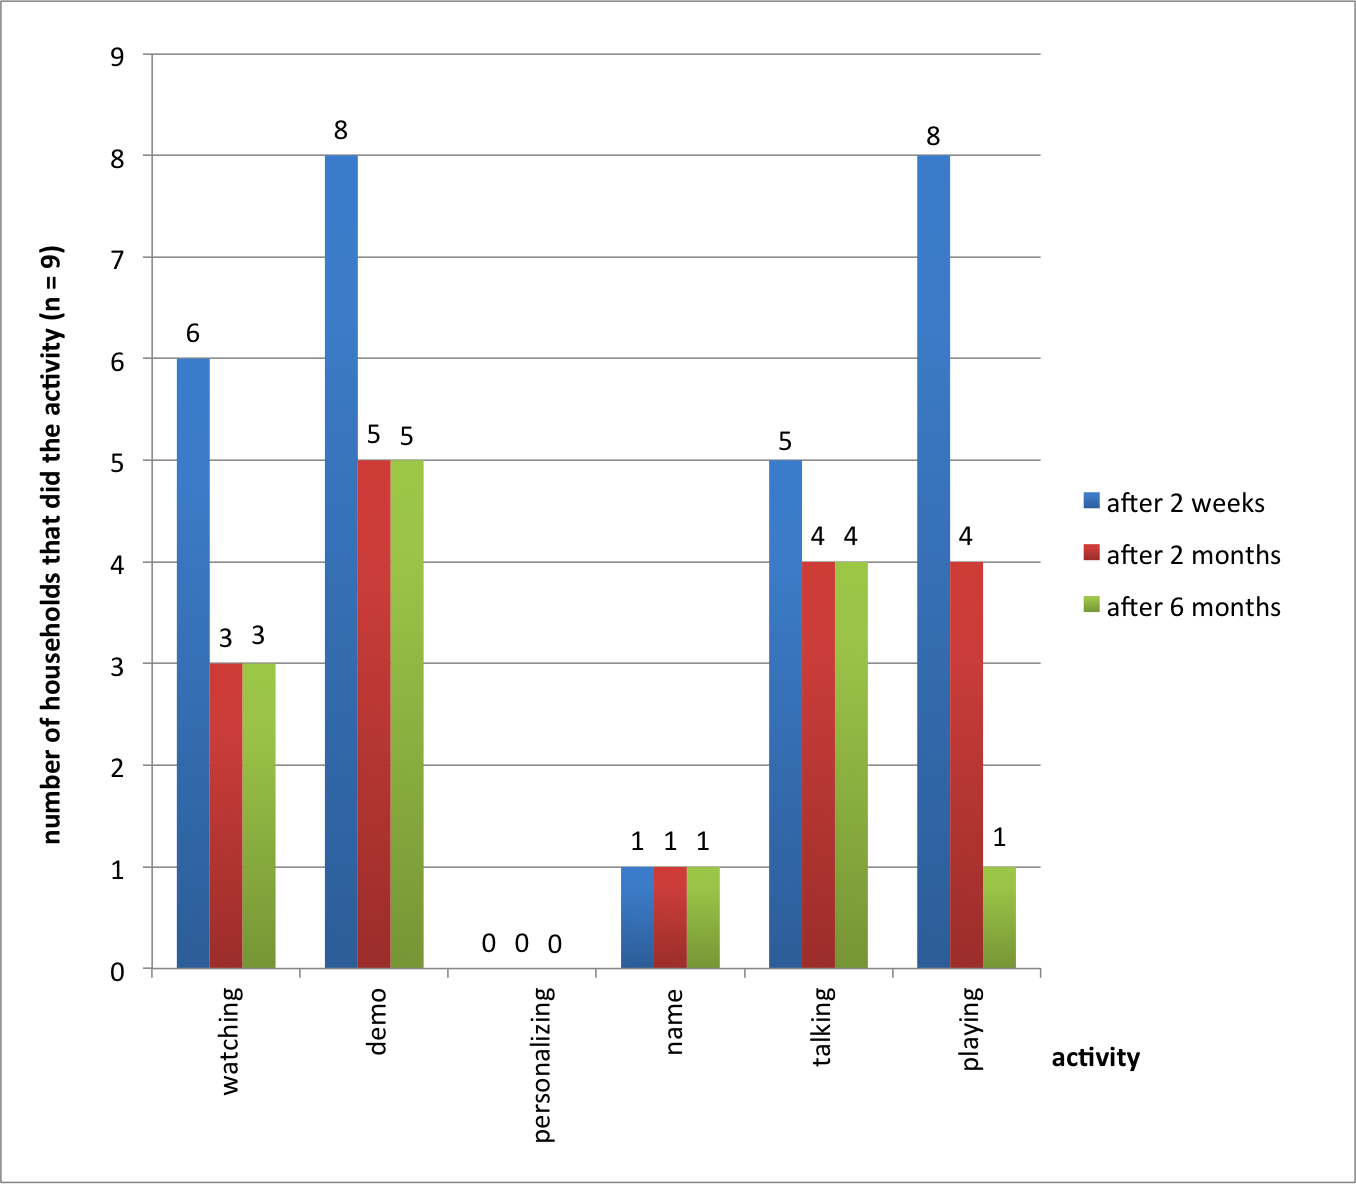
\includegraphics[width=\textwidth]{roomba-activities.png}
                \caption{Activities related to Roomba, n = 9 households}
                \label{fig:roomba-activities}
        \end{subfigure}%
        \hspace{0.5cm} 
        \begin{subfigure}[t]{0.48\columnwidth}
                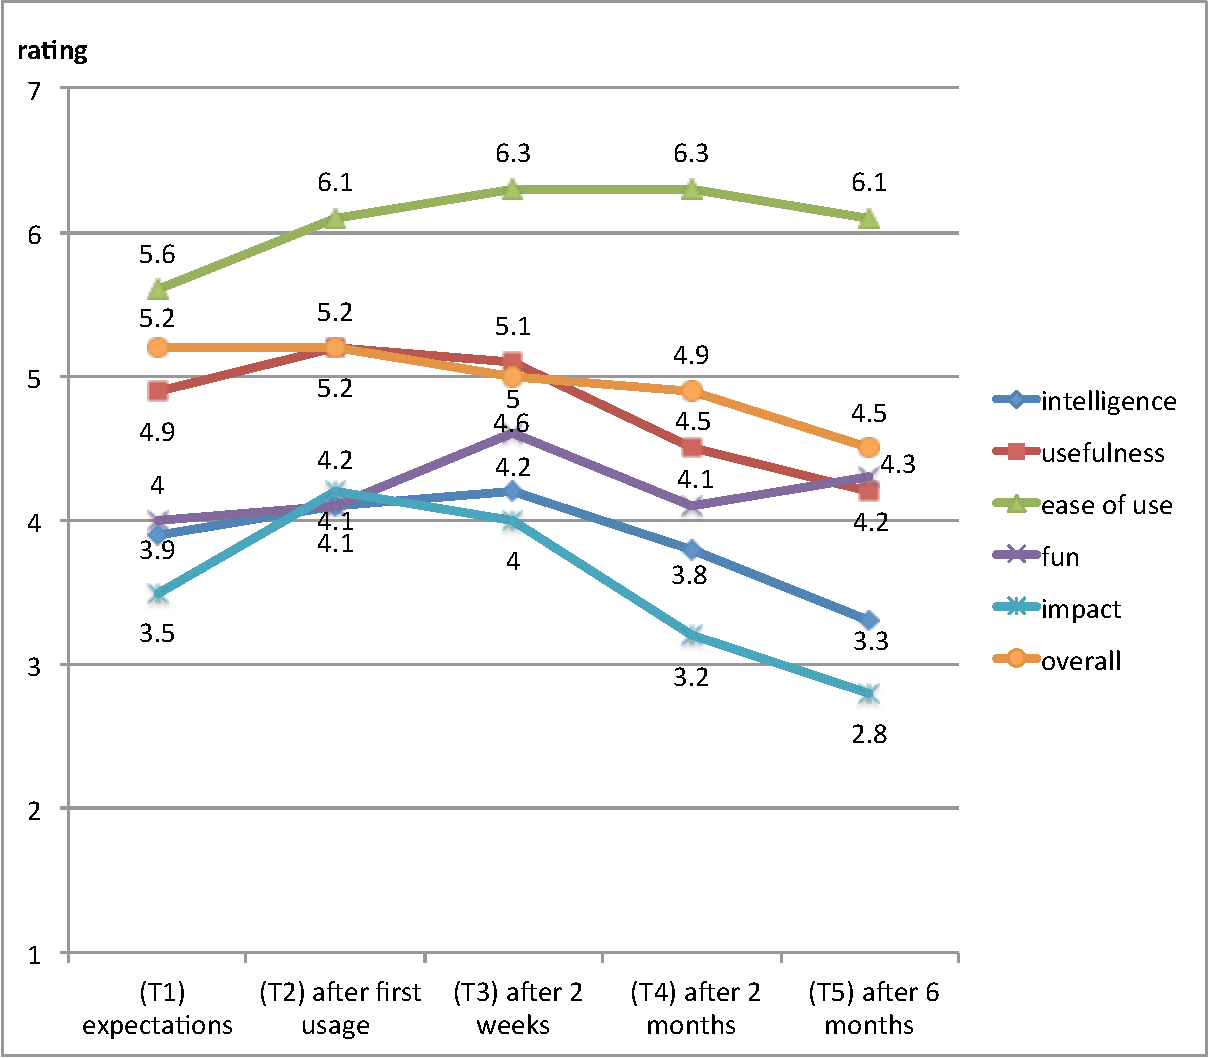
\includegraphics[width=\textwidth]{roomba-perception.pdf}
                \caption{People's perception of Roomba, n = 15 participants}
                \label{fig:roomba-perception}
        \end{subfigure}
    \caption{Usage and perception of the Roomba vacuum-cleaning robot over a 6 months period. Qualitative data suggest that people's activities related to the robot as well as their perception of the robot change over time.}
    \label{fig:roomba}
\end{figure}

Figures~\ref{fig:roomba-activities} and~\ref{fig:roomba-perception} give a first
perspective on how naive users interact and perceive robots over a long period
of time. Here, \emph{Roomba} vacuum cleaning robots were given to nine
households for a 6-months period. The aim was to explore how people use and
perceive the robot over time, and how they generally live with the Roomba in
their home. At various time points, users were asked to rate their perception of
different features of the robot on a 7-point rating scale. As
Figure~\ref{fig:roomba-perception} shows, some features remained stable over
time (\emph{ease of use} and \emph{fun}), and others decreased: the perceived
\emph{usefulness}, \emph{intelligence} and \emph{impact} on their household.
\emph{intelligence} and \emph{impact} reflect the cognitive engagement of the
user towards the machine: we can assume that one does not care to engage in a
(cognitive) interaction with an artifact perceived as non-intelligent and with
no impact on one's life (and the level of activity pictured in
Figure~\ref{fig:roomba-activities} qualitatively confirms this intuition). Even
if one can argue that the Roomba is not designed to foster interaction, it
raises a first question: how to sustain engagement between a robot and a human
over a long period of time? And, as a pre-requisite to answer, do we actually
understand the psychological phenomenon, and can we effectively account for the
dynamics of these interactions?

Those questions are certainly not new, but paradoxically, while anthropomorphism
is a commonly discussed trait of human-robot interaction, it appears
that we lack formal grounds and models that would account for the long-term
dynamics of these interactions.

\begin{figure}[h!]
        \centering
        \begin{subfigure}[b]{0.48\columnwidth}
                \centering
                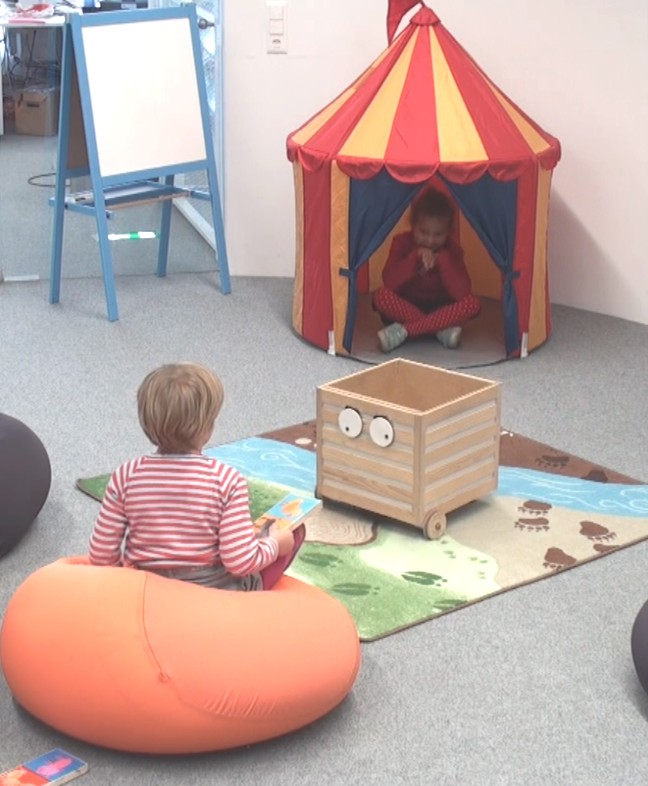
\includegraphics[width=0.75\textwidth]{ranger}
                \caption{Interaction scenario of the \emph{Ranger} domino study: the robot toy box Ranger transports domino tiles between the two children}
                \label{fig:ranger-expe}
        \end{subfigure}%
        \hspace{0.5cm}
        \begin{subfigure}[b]{0.48\columnwidth}
            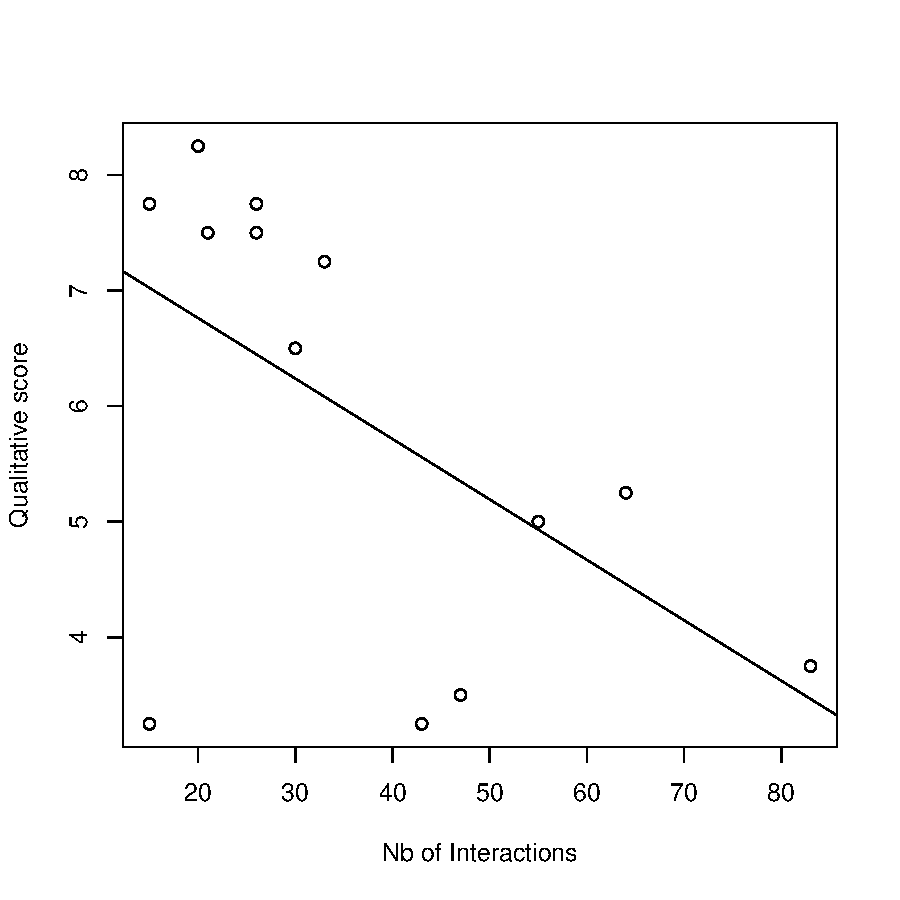
\includegraphics[width=\textwidth]{ranger-interactions-vs-qualitative-score}
            \caption{We found a significant negative correlation ($p=0.048$) between the
    number of interactions and the qualitative anthropomorphic projections. n = 13 groups}
            \label{fig:qualitative-score}
        \end{subfigure}
        \caption{Children`s interaction with Ranger, and their anthropomorphic projections onto the robot. Overall, large variations of both children`s behavior and their perception of the robot were found but seemed to be correlated to each other.}
    \label{fig:ranger}
\end{figure}

%\fixme{It was written as caption of fig:ranger: ``Level of interaction with a semi-anthropomorphic robot is \emph{not} a predictor of anthropomorphic projections.'' Comment JF: this statement does not make sense to me as we found a significant negative correlation between the two.}

Figure~\ref{fig:qualitative-score} calls for other initial remarks. This diagram
shows data from a (yet unpublished) study in which 13 pairs of children (4-5 years old)
played for about 20 minutes a Domino game with a robot toy box (the robot was tasked to
carry domino pieces from one child to the other, Figure~\ref{fig:ranger-expe}).
The $x$-axis represents the number of social interactions between the children
and the robot (like talking to the robot or showing objects), based on video annotations. On
the $y$-axis, we have a synthetic qualitative measurement of anthropomorphic
projections onto the robot, based on two interviews with the children. The correlation between both these
values is significantly \emph{negative}: the more the children engaged into
interaction, the less prone to anthropomorphic projections they were. This
diagram also highlights an interesting cluster of children who did not interact
much with the robot, and still reported a strong anthropomorphic perception of
the robot.

These results may seem counter-intuitive at first sight, and illustrate that the
mechanisms that relate anthropomorphism to adoption and engagement are
non-trivial. In section~\ref{sec:cognition-neuroscience}, we sketch a model of
the cognitive correlates of anthropomorphism that partially account for these
results.


\subsection{Towards a formal understanding of anthropomorphism}

These first remarks lead to the main question we attempt to address in this
article: how can we understand \emph{anthropomorphism} as a whole, \hl{and in such a
way that is support improved human-robot interactions?}\fixme{JF: something's wrong with this sentence}

We propose to discuss anthropomorphism from three
complementary perspectives: 

%Based on an extensive literature review~\citep{fink_anthropomorphism_2012},
%several field and lab studies previously mentioned, and insights from the
%cognitive neuroscience, we propose to discuss anthropomorphism from three
%complementary perspectives.

First, by reviewing what anthropomorphism actually \emph{means}:
besides an \emph{artifact-centered} understanding that explains anthropomorphism from the human-like design of the non-human artifact, it seems important to explicit the social component, namely a \emph{human-centered} understanding, of anthropomorphism.

Second, we propose a model, called the \textit{Dynamics of Anthropomorphism} to understand how anthropomorphism evolves over time ~\citep{lemaignan2014dynamics}.
These dynamics are non-monotonic, and effects like the
\emph{novelty effect} play here a key role.

Finally, we adopt a third perspective on anthropomorphism by investigating its
\emph{cognitive correlates}. Several studies previously showed that we build
instinctive bonds with robots as soon as we attribute animacy, and we also know
from social psychology some of the mechanisms that lead to
\emph{familiarization}. We attempt here to ``connect the dots'', in order to
build a practical model of the cognitive stages we encounter in human-robot
interaction.


%\paragraph{Two hypotheses}
Our research question also translates to two
hypotheses, which structure the reflections of this article:

\begin{enumerate} 
\item ~A person's tendency to anthropomorphize a robot
    is based on several factors, including (but not limited to) (1) the
    design of the robot, (2) the personal characteristics of the human user,
    and (3) the context and situation of use. For instance, a social context
    and purpose of the robot increase anthropomorphism: \textit{anthropomorphism
    as a multi-factor phenomenon}.

\item ~A person's tendency to anthropomorphize a robot
    evolves in a non-linear way over time and with growing experience that the
    person has with the robot. For instance, a more experienced user will
    perceive the robot as more familiar and predictable, and in turn
    anthropomorphizes the robot less: \textit{anthropomorphism as a dynamic
    phenomenon}.

\end{enumerate}

\subsection{Article overview}

%\begin{inparaenum}[\itshape 1)\upshape]

The remainder of this article is organized as follows.
According to the three perspectives that we take, 
we first (in Section
%\ref{sec:overview-studies}, we give a brief overview on the various studies that
%we conducted to investigate anthropomorphism, namely \item the Roomba study,
%\item the Forum study, \item the Ranger domino study. Next, Section
\ref{sec:anthropomorphism}) aim to establish a common ground in the
understanding of anthropomorphism. We review literature from several relevant domains and integrate the different explanations into an understanding of
anthropomorphism as a multi-factor phenomenon.
Based on this, Section~\ref{sec:our-ideas} introduces our initial model of the
\textit{Dynamics of Anthropomorphism}. This model describes the variances
and dynamics of people's tendency to anthropomorphize an artificial agent,
such as a robot. 
Then Section \ref{sec:cognition-neuroscience} presents a
cognitive and neuroscience perspective on anthropomorphism to consolidate
our considerations and the proposed model.
This is followed by a discussion
about the limitations of our approach (Section \ref{sec:discussion}) and the
existing and alternative ways to measure anthropomorphism in human-robot
interactions.
Finally, Section \ref{sec:conclusion} concludes this article
and offers starting points for further research on anthropomorphism and the
effect of the human-like design approach in robotics.

%\end{inparaenum}

%
%%%%%%%%%%%%%%%%%%%%%%%%%%%%%%%%%%%%%%%%%%%%%%%%%%%%%%%%%%%%%%%%%%%%%%%%%%
%%
%%
%%
%%		OVERVIEW ON OUR STUDIES
%%
%%
%%
%%%%%%%%%%%%%%%%%%%%%%%%%%%%%%%%%%%%%%%%%%%%%%%%%%%%%%%%%%%%%%%%%%%%%%%%%%
%
%\section{Studying anthropomorphism in HRI}
%\label{sec:overview-studies}
%
%In this section we give a brief overview of the studies that we conducted to
%investigate anthropomorphism in human-robot interaction. Note that it was not
%the main purpose of these studies to analyze in detail the effect of different
%dimensions human-likeness of a robot on the user's perception of and interaction
%with the robot. Each of these studies were motivated also by other research
%questions, and we encourage the reader to refer to our other main publications
%about these studies for more details.
%
%
%\subsection{Roomba study: how people live with a vacuum cleaning robot}
%
%We openly explored long-term interactions between human users and a domestic
%service robot in a 6-months lasting ethnographic study~\citep{fink_living_2013}. 
%We gave a commercially
%available vacuum cleaning robot (iRobot's Roomba, see Figure
%\ref{fig:aibo-roomba-ipad} middle) to nine households. 
%%in the French speaking
%%part of Switzerland. 
%%The fairly diverse sample of households consisted of 2
%%single homes, 1 couple, and 6 families with children in their home. In total,
%%this summed up to 30 participants: 15 adults (26-71 years old, mean age 43.6
%%years), and 15 children (6 months to 18 years old). During the 6 months, each
%%household was visited 5 times to conduct interviews and make field observations
%%in the households. Moreover, during several weeks, households were asked to fill
%%in a diary to report the usage of the robot and other cleaning activities.
%Hereafter, we refer to this study as the ``Roomba study''. It is one of very few 
%long-term human-robot interaction studies in the domestic environment. 
%In the following, we present findings in respect of two aspects: First, we
%qualitatively describe what kinds of anthropomorphic interactions between
%participants and the robot were observed and outline how these interactions
%evolved over time.  Second, we present people's perception of human-likeness and
%social capabilities of the robot and how this perception changed over
%time.
%
%%\footnote{\hl{note that these two different kinds of data
%%(behavior/interaction and perception) already show that we try to measure
%%anthropomorphism from these two angles!}}
%
%%The main goal of this study was to explore how households live with a vacuum
%%cleaning robot over an extended period of time. We wanted to analyze how the
%%usage of and interaction with the robot evolve over time, and to identify
%%adoption phases as well as factors that impact on the long-term acceptance of
%%service robots in homes.
%
%
%\subsubsection{Anthropomorphic interactions with the robot\\}
%
%It has been described in several previous studies of the Roomba that users tend
%to engage in a variety of non-cleaning activities associated with the robot,
%including, but not limited to, naming, ascribing personality and gender
%\citep{forlizzi_service_2006,forlizzi_how_2007,krumm_my_2007,sung_domestic_2010}.
%\cite{sung_housewives_2008} carried out a survey among 379 Roomba users to
%investigate how common these activities are. The authors concluded that overall,
%respondents had relatively low rates of treating Roomba as a living entity.  
%Similarly, in our long-term study of the Roomba in homes, we found that only few 
%people tended to interact in an anthropomorphic or human-social way with their 
%vacuum cleaning robot and that this effect did not sustain. Overall, our data 
%suggest that the anthropomorphic effect and the social
%impact of a functional robot on a household are rather marginal.
%%There were just few instances of people anthropomorphizing the robot and
%%interacting with it in a human-social way. More importantly, overall, these
%%anthropomorphic interactions with the robot did not last but seemed to be
%%somehow related to the novelty of the robot.
%
%We categorized several interactions and actions with the robot as
%anthropomorphic or human-social (in a broader sense). 
%%Examples of what we categorized as somehow social and anthropomorphic
%%(human-like) interactions with the robot include \textit{watching} the robot
%%for fun, giving a \textit{demo} of the robot to guests / visitors, taking a
%%\textit{photo/video} of the robot, \textit{personalizing} the robot, giving a
%%\textit{name} to the robot, \textit{talking} to the robot using direct speech,
%%\textit{playing} with the robot, and making \textit{adjustments} to the home
%%due to the robot. 
%Figure \ref{fig:roomba-activities} shows how many of the 9 households engaged
%in these activities during the 6 months when the study was conducted. 
%
%%\begin{figure}
%%    \centering
%%    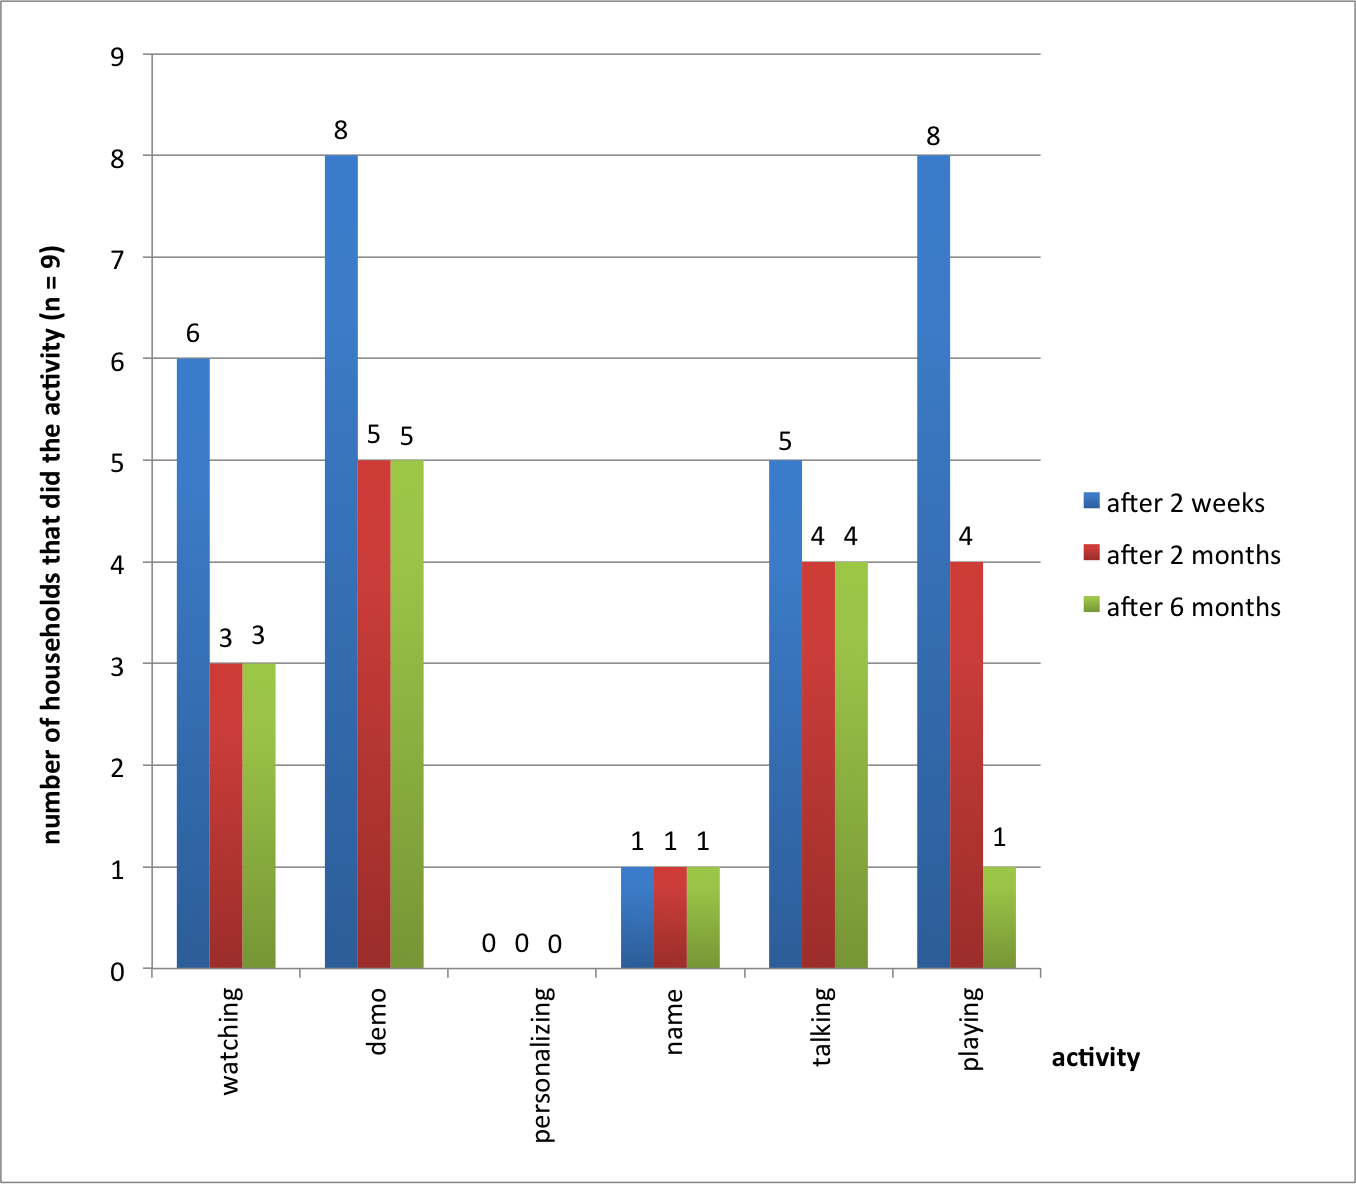
\includegraphics[width=0.5\columnwidth]{roomba-activities.png}
%%    \caption{Activities with the robot over time, n = 9 households. This bar
%%        chart shows how many of the 9 households carried out different kinds of
%%        anthropomorphic / social activities with and related to the robot at 3
%%        time points during 6 months. Activities include \texttt{watching} the
%%        robot for fun, giving a \texttt{demo} of the robot to guests / visitors,
%%        \texttt{personalizing} the robot, giving a \texttt{name} to the robot,
%%        \texttt{talking} to the robot, \texttt{playing} with the robot.
%%        Participants were asked to report on these activities at 3 time points
%%        after the robot was deployed in their home: after 2 weeks, after 2 months,
%%        and after 6 months.} 
%%
%%\label{fig:roomba-activities}
%%\end{figure}
%
%\begin{figure}
%        \centering
%        \begin{subfigure}[b]{0.48\columnwidth}
%                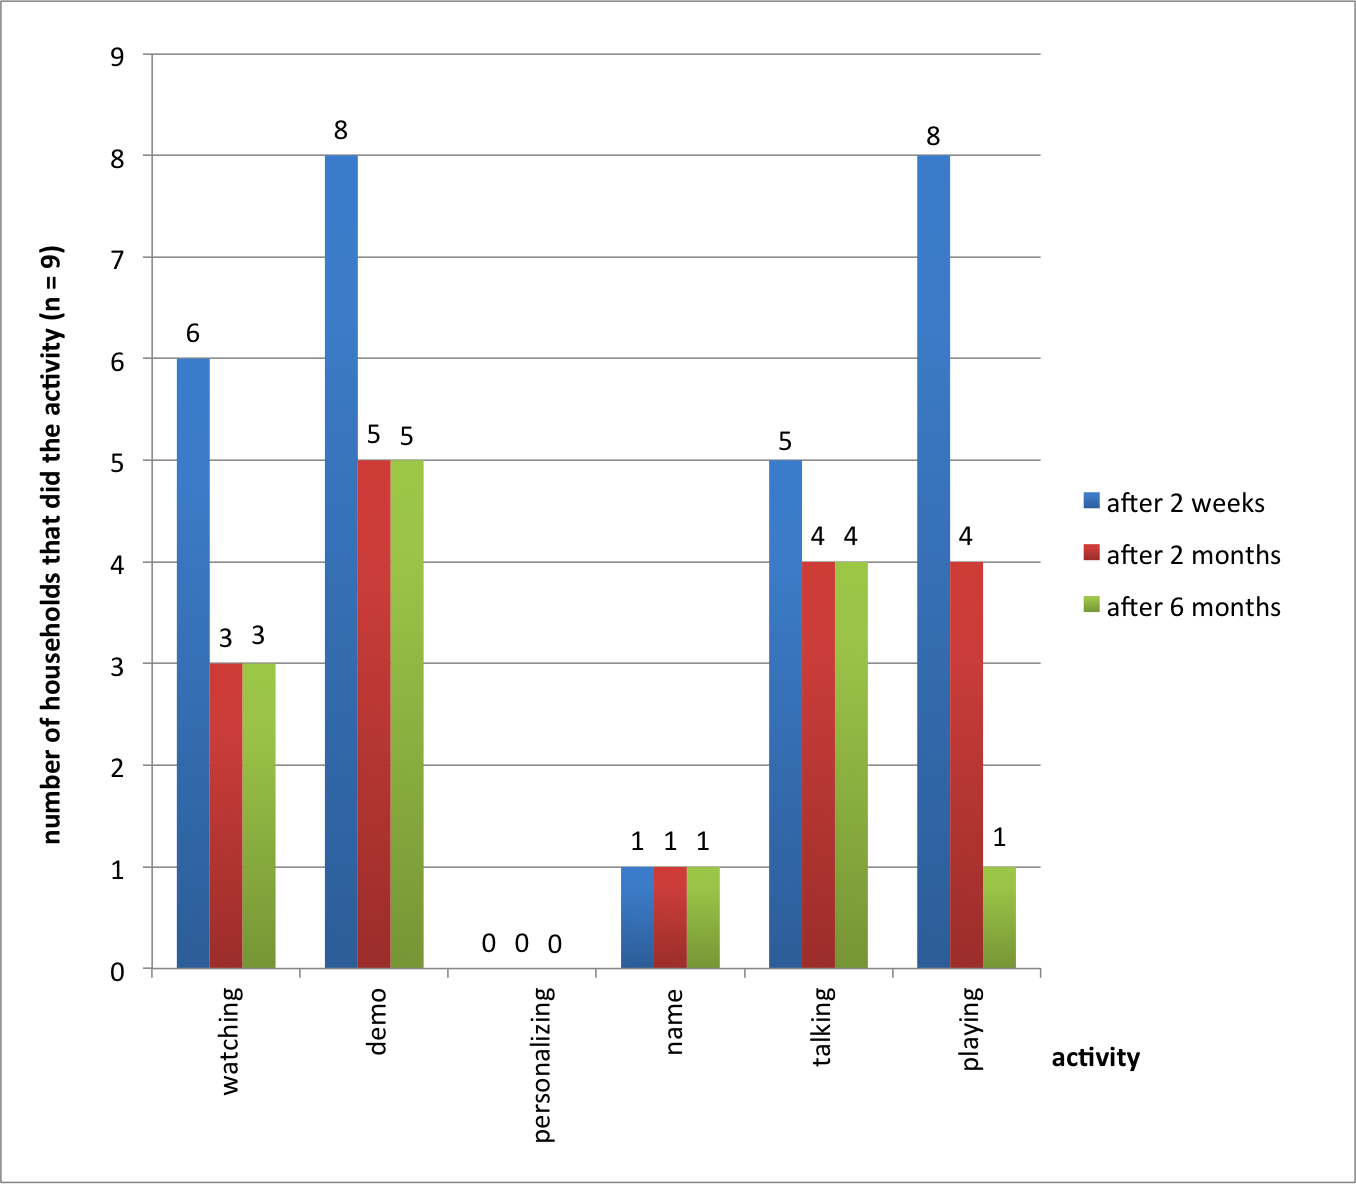
\includegraphics[width=\textwidth]{roomba-activities.png}
%                \caption{Roomba activities}
%                \label{fig:roomba-activities}
%        \end{subfigure}%
%        ~ %add desired spacing between images, e. g. ~, \quad, \qquad etc.
%          %(or a blank line to force the subfigure onto a new line)
%        \begin{subfigure}[b]{0.48\columnwidth}
%                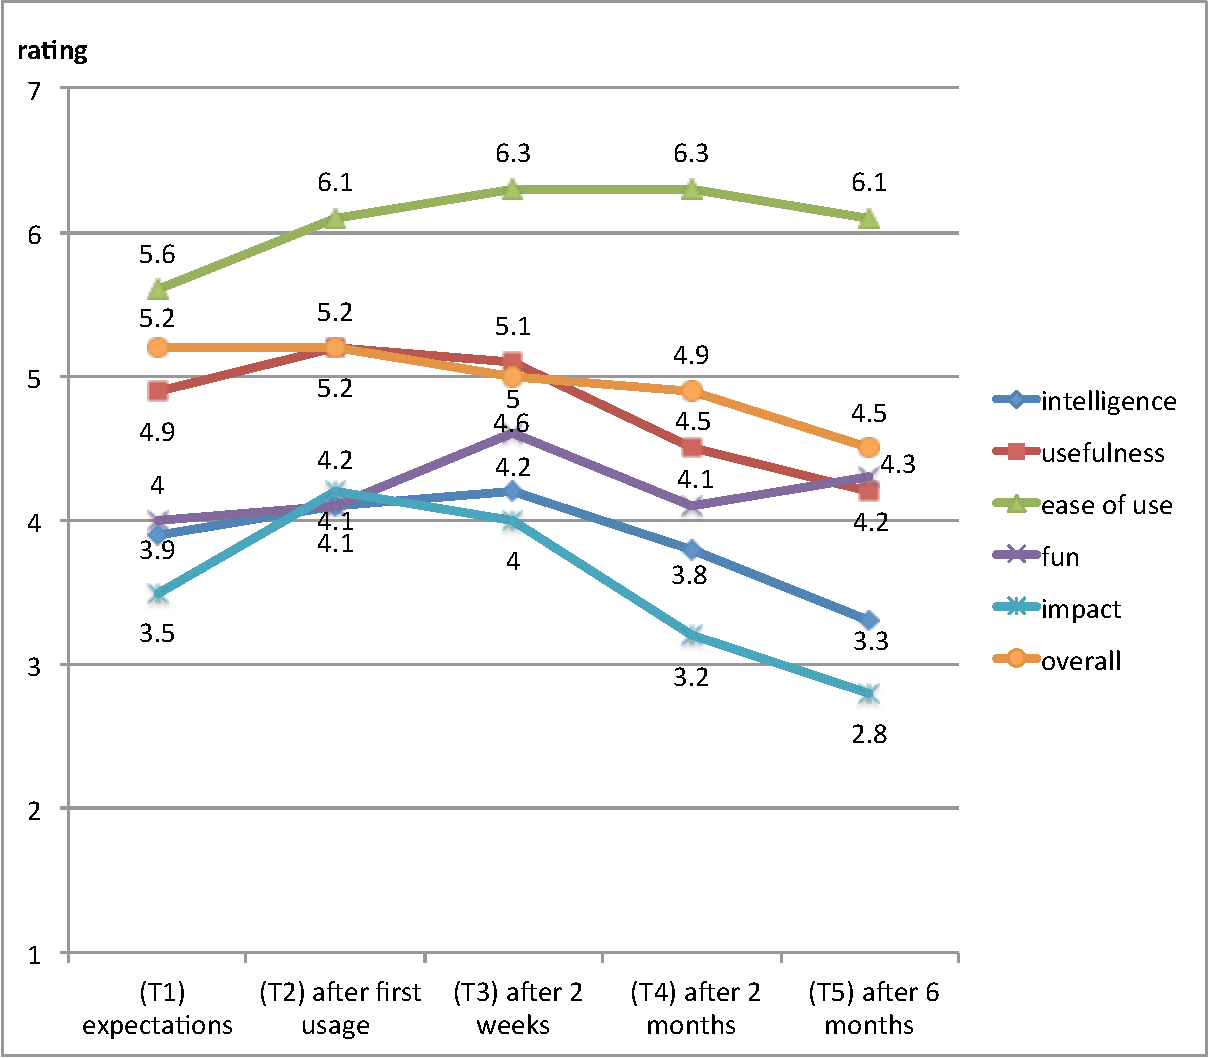
\includegraphics[width=\textwidth]{roomba-perception.pdf}
%                \caption{Roomba perception}
%                \label{fig:roomba-perception}
%        \end{subfigure}
%        \caption{\textbf{The Roomba study: Long-term interaction with a robot.\\}
%    \textbf{a)} Activities with the robot over time, n = 9 households. This bar
%        chart shows how many of the 9 households carried out different kinds of
%        anthropomorphic / social activities with and related to the robot at 3
%        time points during 6 months. Activities include \texttt{watching} the
%        robot for fun, giving a \texttt{demo} of the robot to guests / visitors,
%        \texttt{personalizing} the robot, giving a \texttt{name} to the robot,
%        \texttt{talking} to the robot, \texttt{playing} with the robot.
%        Participants were asked to report on these activities at 3 time points
%        after the robot was deployed in their home: after 2 weeks, after 2 months,
%        and after 6 months.\\
%	\textbf{b)} People's perception of the robot over time, n = 15 participants.
%    		This line chart shows how people's perception of the robot evolves over
%    		time. At 5 time points people were asked to rate the robot according to the
%    		following aspects: the perceived \texttt{intelligence} of the robot, the
%    		perceived \texttt{usefulness}, the perceived \texttt{ease of use}, how much
%    		\texttt{fun} it was to use the robot, how far they found the robot had an
%    		\texttt{impact} on their household, and their {overall} impression of it.}
%    		\label{fig:roomba-study}
%\end{figure}
%
%
%\paragraph*{Watching the robot for fun.} We categorize watching a robot for fun
%as an entertaining, emotional activity, reflecting a feeling of empathy for the
%robot. In \cite{sung_housewives_2008} survey, 73~\% of the participants reported
%to watch their Roomba running for fun. While in the beginning of our study, also
%a quite high proportion (6 of 9 households) reported to watch the robot for fun,
%after 2 and 6 months the number of households that engaged in this activity
%decreased by half. 
%
%\paragraph*{Giving a robot demo to visitors.} It is somehow natural that owners
%of innovative devices show the device to others and ask for their opinion about
%it \citep{rogers_diffusion_1995}. However, this activity suggests that the robot
%is presented as a new part of the household to visitors.
%\cite{sung_domestic_2010} described that a vacuum cleaning robot can serve as a
%mediator and encourage social interaction among people. We categorize giving a
%demo of the robot to visitors / guests as such an activity. During the first 2
%weeks with the robot 8 of 9 households in our study showed their robot to
%others, and still after 2 and 6 months 5 of the households engaged in this
%activity. This number is more or less in accordance with the 57~\% of survey
%respondents who stated to give demonstrations to others
%\citep{sung_housewives_2008}.
%
%%\paragraph*{Taking photos / videos of the robot.} How far taking a photo or
%%video of a robot can be seen as an anthropomorphic interaction is questionable.
%%However, it reflects the fact that the robot is observed by the user who for
%%some reason is motivated to record the event. The number of households that
%%took a photo or video of the robot decreased over time from 5 households in the
%%beginning to 1 household after 6 months.
%
%\paragraph*{Personalizing the robot.} It has been found that people are
%motivated to personalize technology as a form of self-expression (identity
%projection) or when they use a technology a lot and know how to customize it
%(technical identity projection) \citep{blom_personalization:_2000}. Though
%\cite{sung_pimp_2009} found that some Roomba users who were given a
%customization toolkit personalized their Roomba, none of the users in her study
%who was \textit{not} given this toolkit personalized their Roomba. Also in our
%study none of the 9 households engaged in a personalization activity.
%
%\paragraph*{Giving a name to the robot.} Giving a name to an artificial agent
%reflects a certain kind of personal relationship to the agent. By naming a
%robot, it is not anonymous anymore, and might be perceived as a moral agent. As
%such, naming an artificial agent can be classified as anthropomorphizing this
%agent. It further suggests that the agent is talked to directly. Though more
%than 23~\% of the survey participants in \cite{sung_housewives_2008} study
%reported to name their Roomba, only 1 of 9 households in our study did so. 
%
%\paragraph*{Talking directly to the robot.} Using direct speech toward an object
%or artificial agent that does not have the ability to recognize and process
%speech (such as verbal comments) or other sound cues, is an interesting
%phenomenon which can be classified as an anthropomorphic interaction. Whereas
%only 11~\% of the survey respondents in \cite{sung_housewives_2008} study
%reported to talk to their robot, around half of the households engaged in this
%activity and the proportion did not notably decrease over time. 
%
%\paragraph*{Playing with the robot.} In our study, it were mostly children who
%engaged in playing with the robot, however, most of them stopped doing so after
%some time. The number of household playing with their Roomba decreased from 8
%when asked after 2 weeks with the robot, to 4 households after 2 months, and 1
%household after 6 months. In \cite{sung_housewives_2008} survey, 37~\% of the
%Roomba owners reported to play and experiment with their robot.\\ 
%
%%\paragraph*{Making adjustments to the home due to the robot.} To help Roomba
%%clean, \cite{sung_housewives_2008} found in an online survey that about half of
%%the 379 participants made physical modifications to their homes. This process
%%is referred to as \textit{roombarization}, and it seems to be a unique aspect
%%of adopting a domestic service robot. In our study, almost all the households
%%made adjustments when they used the robot for the first time in front of us.
%%However, during the first two weeks with the robot, only 3 households reported
%%to have adjusted something due to the robot, and after 6 months it was only 1
%%household that still engaged in this activity. This decrease is, however,
%%logical since after some time most people had done all the necessary
%%adjustments to enable the robot show a good performance.
%
%%\paragraph*{Emerging anthropomorphic interactions.} Another, from our side more
%%unexpected interaction that we would describe as somehow anthropomorphic, is
%%what we call \textit{``collaborative cleaning''} with the robot. In the initial
%%phase of the study, some people spontaneously helped the robot to clean by
%%either picking up crumbs from the floor themselves or pushing it right in front
%%of the robot. Another way of collaborating with the robot we observed was to
%%help it go everywhere by spontaneously putting up the trash bin or the carpet
%%in the bathroom (things that are not just lying around and need to be cleaned
%%up). However, the activity of collaborative cleaning faded out soon, and we
%%suspect it was encouraged by the novelty of the robot.\\
%
%Overall, Figure \ref{fig:roomba-activities} shows that as time goes by, less
%households engage in the before-mentioned non-cleaning activities with the
%vacuum cleaning robot: after 2 weeks, on average, 4.67 of 9 households engage in
%a human-like activity with the robot; after 2 months, the value decreases to
%2.83, and after 6 months to 2.3. Our interpretation is that the nature of
%human-robot interaction changes over time. More concretely, we suspect  that
%anthropomorphic / human-social interactions with the robot become less over
%time, and that only with some people these interactions sustain.
%
%
%\subsubsection{Perception of anthropomorphic characteristics of the robot\\}
%
%We also studied people's perception of the robot, and how it evolved over time
%(see Figure \ref{fig:roomba-perception}). The main idea was to find out which of
%the perceived attributes could be related to how far the robot was integrated in
%the household as a cleaning tool. Concerning anthropomorphism, we included
%\textit{perceived intelligence} and experienced \textit{fun} when using the
%robot as indicators for the perception of human-likeness in the robot.\fixme{JF: Severin, you also mentioned impact as one factor. Please include it here below as another paragraph.}
%
%%\begin{figure}
%%    \centering
%%    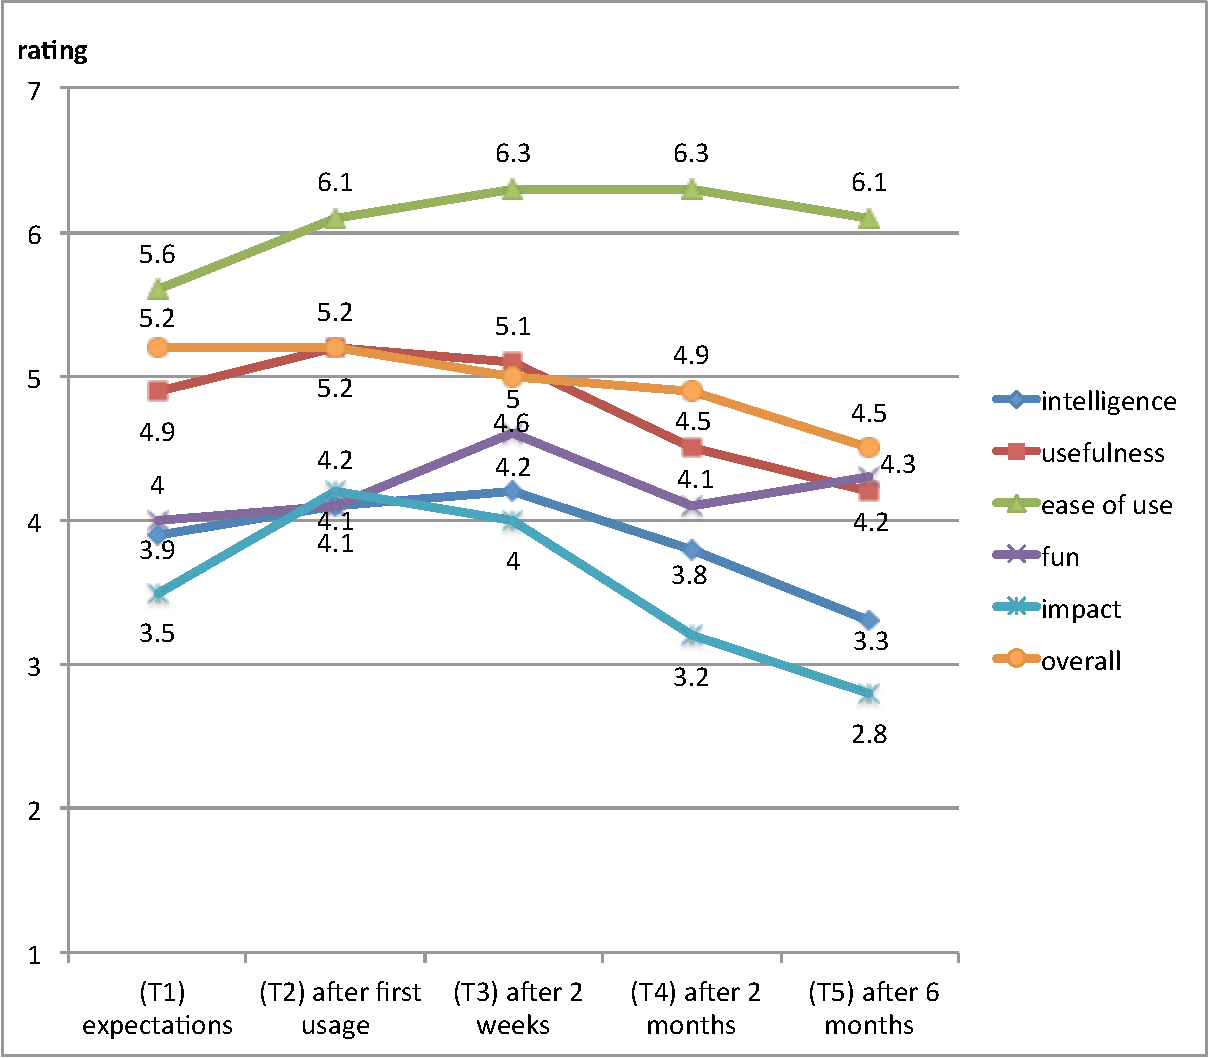
\includegraphics[width=0.5\columnwidth]{roomba-perception.pdf}
%
%%    \begin{tikzpicture}[scale=0.5, y = 2cm]
%%    %axis
%%    \draw (0,0) -- coordinate (x axis mid) (20,0);
%%    \draw (0,0) -- coordinate (y axis mid) (0,7);
%%    %ticks
%%    \foreach \x in {0,4,...,20}
%%        \draw (\x,1pt) -- (\x,-3pt);
%%    \foreach \y in {1,...,7} 
%%        \draw[black!20] (20,\y) -- (-3pt,\y);
%%    \foreach \y in {1,...,7} 
%%        \draw (-3pt, \y) node[anchor=east] {\y}; 
%%    %labels
%%    \node[below=0.8cm] at (x axis mid) {People's perception (n = 15)};
%%    \node at (2, -0.4) {\tiny expectations};
%%    \node[align=center] at (6, -0.4) {\tiny after\\ \tiny first usage};
%%    \node[align=center] at (10, -0.4) {\tiny after\\ \tiny 2 weeks};
%%    \node[align=center] at (14, -0.4) {\tiny after\\ \tiny 2 months};
%%    \node[align=center] at (18, -0.4) {\tiny after\\ \tiny 6 months};
%%
%%    \draw[dashed, black!50] (6,0) -- (6,7) node[sloped, below, pos=0.25] {\tiny novelty effect};
%%
%%    \draw[ultra thick, red!50] (2,5.6) -- (6,6.1) -- (10,6.3) -- (14,6.3) -- (18,6.1) node at (15,6.5) {\tiny \it ease of use};
%%    \draw[ultra thick, purple] (2,4.9) -- (6,5.2) -- (10,5.1) -- (14,4.5) -- (18,4.2) node at (3,4.7) {\tiny \it usefulness};
%%    \draw[ultra thick, blue!50] (2,4) -- (6,4.1) -- (10,4.6) -- (14,4.1) -- (18,4.3) node at (16,4) {\tiny \it fun};
%%    \draw[ultra thick, green!50] (2,3.9) -- (6,4.1) -- (10,4.2) -- (14,3.8) -- (18,3.3) node at (19,3.5) {\tiny \it intelligence};
%%    \draw[ultra thick, orange] (2,3.5) -- (6,4.2) -- (10,4) -- (14,3.2) -- (18,2.8) node at (14,2.7) {\tiny \it impact};
%%
%%    \draw[ultra thick, dashed] (2,5.2) -- (6,5.2) -- (10,5) -- (14,4.9) -- (18,4.5) node at (14,5.3) {\tiny \it overall};
%%
%%    \end{tikzpicture}
%
%
%%    \caption{People's perception of the robot over time, n = 15 participants.
%%    This line chart shows how people's perception of the robot evolves over
%%    time. At 5 time points people were asked to rate the robot according to the
%%    following aspects: the perceived \texttt{intelligence} of the robot, the
%%    perceived \texttt{usefulness}, the perceived \texttt{ease of use}, how much
%%    \texttt{fun} it was to use the robot, how far they found the robot had an
%%    \texttt{impact} on their household, and their {overall} impression of it.}
%%
%%    \label{fig:roomba-perception}
%%\end{figure}
%
%\paragraph*{Perceived intelligence.} On a scale from 1-7, people were not sure
%about how intelligent they should expect the robot to be (mean value 3.9). The
%rating did not change much and not significantly over time (average ratings
%between 3.3-4.2) \citep{fink_living_2013}. Interestingly, at all five time
%points, male participants rated the robot as more intelligent (average 4.5) than
%females (average 3.4), however, this difference was not significant. When asked
%why they thought Roomba possesses intelligence, men more often referred to the
%'robot side' of Roomba: its abilities to detect and avoid obstacles, stairs, and
%being able to recharge itself. Contrary, women referred to its rather limited
%vacuuming performance and found it was not as intelligent because \textit{``it
%doesn't see where the dirt is, it sometimes leaves it, it can't be smart!''}.
%This difference in the perception of intelligence of a robot suggests that
%gender,and probably other individual characteristics need to be taken into
%account.
%
%\paragraph*{Experienced fun.} Participants rated the robot as 'somewhat fun'
%(values from 4.0-4.6). There was a qualitative gender difference (not
%significant), in the sense that the experienced fun remained quite stable for
%male participants, whereas it tended to decrease with time for female
%participants. Men described the robot more as a 'fun gadget' than females, who
%referred to it as \textit{``In the end, Roomba is a cleaning tool and it is not
%really fun to use it''}. Again for this aspect, gender seems to play a role in
%how the robot is perceived and experienced.\\
%
%Overall, Figure \ref{fig:roomba-perception} shows that after the first usage of
%the Roomba (T2), most of the perceived constructs slightly decrease (and hence
%are less positively rated) as time goes by. The course is different for the
%perceived \textit{ease of use} of the robot, as participants become more
%experienced with the robot over time. Also, the experienced \textit{fun} does
%not decrease with time.
% 
%
%\subsubsection{Summary Roomba study\\}
%
%In accordance with previous work we also found relatively low rates of users
%treating and perceiving their vacuum cleaning robot as a living (or human-like)
%entity \citep{sung_housewives_2008}. We interpret that it might be the pure
%functional purpose and non human-like form of the Roomba that prevented people
%from anthropomorphizing it. Still, we observed some initial anthropomorphic
%effects, both reflected in interaction with and perception of the robot.
%However, most of the anthropomorphic effects did not last long. One fairly
%stable human-like interaction with the robot was \textit{talking to the robot},
%despite the fact that the robot was not able to recognize and respond to verbal
%statements.
%
%
%\subsection{Forum study: using anthropomorphic expressions to describe a robot}
%
%We investigated the amount and context of anthropomorphic language in three
%online discussion forums about the robotic dog AIBO, the vacuum cleaning robot
%Roomba, and the tablet computer iPad. This was done by means of a content
%analysis of 750 forum posts that were further partitioned in n = 1208 valid
%segments \citep{fink_anthropomorphic_2012}. Hereafter, we refer to this study as
%the "Forum study". The three devices, pictured in Figure
%\ref{fig:aibo-roomba-ipad}, were chosen as they show different designs and
%fulfill different purposes. We would describe (1) AIBO as a zoomorphic /
%pet-like robot that does not have a clear purpose but engages people to play
%with it; (2) Roomba as a mechanical / functional domestic service robot that has
%a practical main purpose (vacuum cleaning) but offers not much of interactivity;
%(3) the iPad as a minimalistic designed interactive (touch-based) technology
%with multiple purposes (both entertainment, and professional / practical use).
%Based on these different characteristics, we made the two following hypotheses
%concerning anthropomorphism:
%
%\begin{enumerate}
%    	\item People engage in a more social and human-like way with a robotic pet compared to a functional robot and a tablet computer, therefore there will be a higher amount of anthropomorphic language in the AIBO and Roomba forum, compared to the iPad forum.
%    	\item As anthropomorphism can be seen as a certain kind of emotional / social relation to an artifact, there will be more anthropomorphic language in forum posts in which the author describes a relation to the device, compared to discussing technological aspects or how the device is used.
%\end{enumerate}
%
%Similar to how \cite{friedman_hardware_2003} analyzed anthropomorphic language
%in online forums, we coded a segment as anthropomorphic when the respective
%device was described in terms of:
%
%\begin{itemize}
%    \item \textit{Life-likeness}, such as being alive or having (parts of) a
%        body, \eg \textit{``she can be reborn since you copied her memory
%        stick''};
%    \item \textit{Emotional states, empathy} or the technology having a
%        \textit{feeling}, \eg \textit{``oh no, poor AIBO''};
%    \item \textit{Gender, personality} or the technology having an
%        \textit{intention}, \eg Roomba \textit{``seems to like to hang around
%        under the sofa''};
%    \item When the author gave the technology a \textit{name}, \eg
%        \textit{``whenever I show Java his pink ball''};
%    \item Being \textit{socially integrated}, such as being a family member, \eg
%        \textit{``I'm considering adding a Roomba to the family''};
%    \item \textit{Metaphorical ways}, \eg Roomba \textit{``sings its victory
%        song when it finishes and docks''}.
%\end{itemize}
%
%In the next paragraphs, we present findings in respect of our two hypotheses:
%anthropomorphic language related to the device, and anthropomorphic language
%related to the topic of the forum post.
%
%\begin{figure}[b]
%    \centering
%    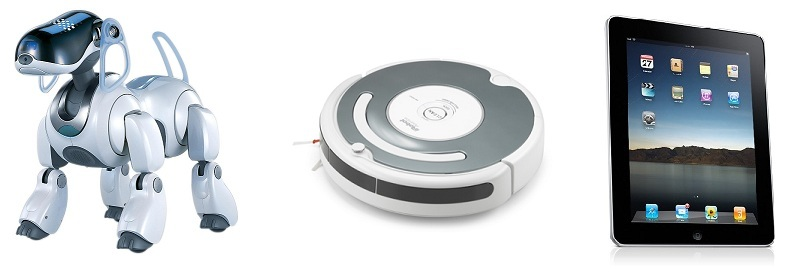
\includegraphics[width=0.5\columnwidth]{aibo-roomba-ipad_2.jpg}
%    \caption{The Sony AIBO robotic dog (left), the iRobot Roomba vacuum-cleaning robot (middle), and the Apple Inc. iPad tablet computer (right) were compared in terms of how far users of these devices use anthropomorphic expressions in online discussion forums about their technology / robot.}
%    \label{fig:aibo-roomba-ipad}
%\end{figure}
%
%%Overall, our analysis revealed that in all three forums, discussions about
%%\textit{technical} aspects of the respective device were most frequent (67.7~\%
%%of all 1208 categorized segments). However there were huge differences between
%%the three devices: \textit{technical} aspects made up 79.9~\% of the discussion
%%in the Roomba forum, compared to 69.9~\% in the AIBO forum, and 55.2~\% in the
%%iPad forum. Another fairly frequently discussed topic concerned the
%%\textit{usage} of the respective device, thus people describing how and for what
%%they use their technology. This topic made up 21.8~\% of all posts, and was most
%%frequent in the iPad forum (35.7~\%), followed by the Roomba forum (15.9~\%),
%%and the AIBO forum (10.7~\%). Last but not least, we defined \textit{relation}
%%as the third topic of interest. Discussions in which people described their
%%relation to the respective device made up 10.5~\% of all posts, and was most
%%frequent in the AIBO forum (19.4~\%), followed by the iPad forum (9.1~\%), and
%%the Roomba forum (4.2~\%). \hl{(if it is getting too much we can leave out this
%%paragraph, it's not crucial, and doesn't say anything about anthropomorphism
%%directly)}
%
%
%\subsubsection{Anthropomorphic language related to the device (design)\\}
%
%A statistical analysis revealed a significant difference for the use of
%anthropomorphism across the three devices \citep{fink_anthropomorphic_2012}. In
%accordance with our first hypothesis, the highest amount of anthropomorphic
%language (56.6~\%) was found in the AIBO forum. In contrast, only 11.7~\% and
%respectively 2.2~\% of the segments in the Roomba and the iPad forum contained
%anthropomorphic expressions.  The data suggests that on a subjective scale of
%perceived human-likeness (or rather life-likeness), Roomba is closer to the iPad
%than to the AIBO, at least in matters of how they are described with words. This
%was a bit against our expectation. Still, the Roomba is an autonomous robot that
%can navigate around the house itself, and we expected this property to enhance
%anthropomorphism. We interpret that here, the physical embodiment of the object
%and how far it resembles a life-like entity determine how far the object is
%anthropomorphized, and as such the robotic dog is anthropomorphized more than
%the functionally designed devices.
%
%
%\subsubsection{Anthropomorphic language related to the topic of conversation\\}
%
%Also in terms of anthropomorphic language related to the topic of conversation,
%a statistical analysis revealed a significant difference
%\citep{fink_anthropomorphic_2012}. The analysis suggests that anthropomorphizing
%happens more when the topic of conversation is \textit{relation}, compared to
%\textit{usage}, and \textit{technical} aspects. This finding is qualitatively
%confirmed when looking at the distribution of anthropomorphic expressions across
%the three topics in the Roomba and iPad forum (with both technologies the
%highest amount of anthropomorphism is in the \textit{relation} topic). However,
%in the AIBO the amount of anthropomorphic segments is highest for the
%\textit{usage} topic.  We interpret that it is the different type of interaction
%/ use context that makes the difference. Contrary to the iPad and the Roomba,
%the AIBO is made to encourage its user in a playful / social interaction, which
%in turn is a typical use context. Further, AIBO has the ability to respond
%intelligently to its user and environment, which might also encourage people to
%ascribe human-like abilities to it while interacting with it.
%
%
%\subsubsection{Summary Forum study\\}
%
%Overall, findings of the content analysis suggest that there are differences in
%people's tendency to use anthropomorphic language, originating form the design
%characteristics of the artifact. A pet-like robot encourages people to use more 
%anthropomorphic expressions when discussing about it in an online forum. However, 
%the difference might also be related to other factors that we did not analyze 
%here (\eg. author's characteristics). Our analysis further shows that the design 
%of the robot seems to more important than the topic of the discussion. 
%Interestingly, not only the physical embodiment
%of the object but also the interaction complexity and purpose of use of the
%object seems to play a role in how far the object is anthropomorphized.
%
%
%\subsection{Ranger domino study: effect of unexpected robot behavior}
%
%The so-called "Ranger domino study" describes a child-robot interaction study
%that we carried out in a fairly controlled lab setting. One of the goals of this
%study was to investigate the effect of unexpected robot behavior on (1) the
%interaction and engagement with robot, and (2) how far children would ascribe
%human-like abilities (\eg intentions, cognitive abilities) to the robot.
%
%13 groups of each two children (n = 26) who were all between 4-5 years old and
%knew each other, were invited to play with the Ranger
%robot toy box \citep{fink2014which} to assemble a domino together. The robot
%was operated by one of the experimenters using the wizard-of-oz technique.
%Ranger was supposed to transport domino tiles between the two children and it
%would do its job correctly for the first 7 runs, bringing each one domino tile to the child. Then, however, the
%robot started misbehaving by not coming over to the child who was calling the 
%robot. Three different experimental conditions were explored using three different 
%types of misbehavior from the robot side:
%Either the robot was \textit{disobeying} and did not come over at all, or 
%the robot got \textit{lost} on its way to the child, or the robot did a 
%\textit{mistake} by first going in another direction but then turning and 
%coming over to the child who had called it.
%According to these three different types of unexpected robot behavior, we 
%expected to observe variations of how far the children perceived the 
%robot in terms of intentionality, and cognitive abilities.
%
%In respect of anthropomorphism, we analyzed two types of data: children's 
%\textit{interaction} with the robot (\eg do they talk to and use gestures 
%toward the robot?, see Figure \ref{fig:interactions-per-run}), and 
%children's \textit{perception} of the robot (\eg do they believe the 
%robot has an own will, feelings, or is able to understand what they 
%say?). The interaction data was analyzed quantitatively after having 
%annotated the video recordings of the interaction. Children's perception 
%of the robot was analyzed in a qualitative way and processed in a 
%qualitative scale (higher values on that scale indicate more 
%anthropomorphism), see Figure \ref{fig:qualitative-score}.
%
%\begin{figure}
%        \centering
%        \begin{subfigure}[b]{0.48\columnwidth}
%                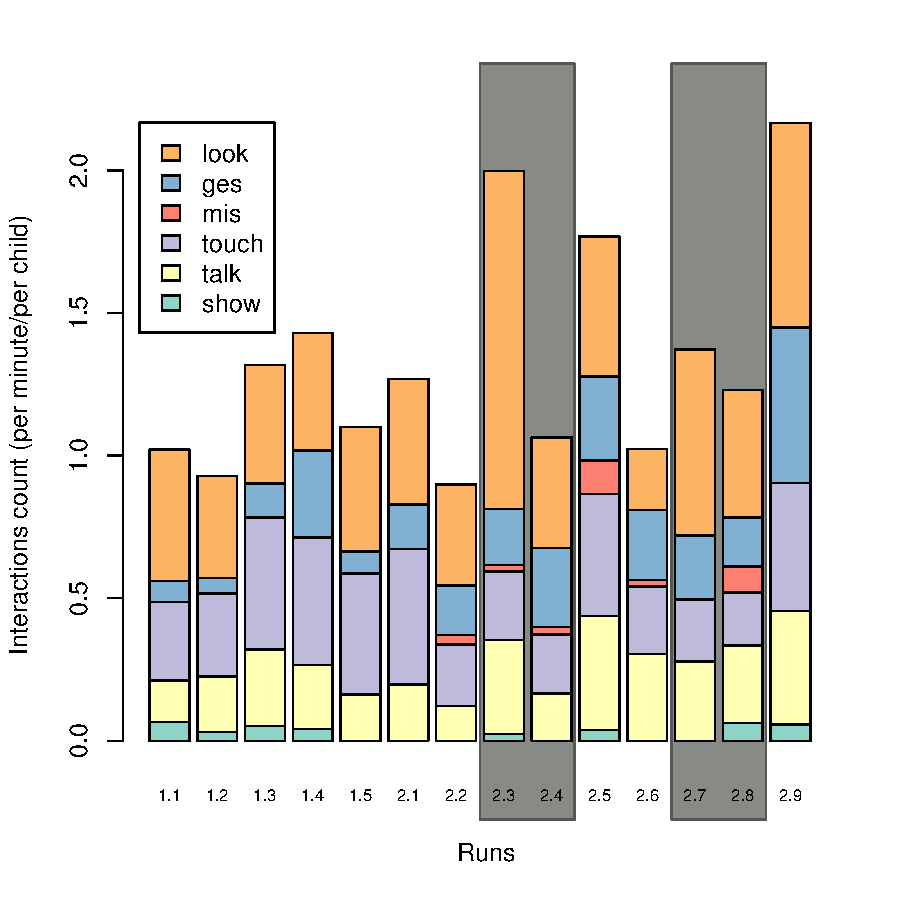
\includegraphics[width=\textwidth]{ranger-interactions-per-runs}
%                \caption{Interactions per run}
%                \label{fig:interactions-per-run}
%        \end{subfigure}%
%        ~ %add desired spacing between images, e. g. ~, \quad, \qquad etc.
%          %(or a blank line to force the subfigure onto a new line)
%        \begin{subfigure}[b]{0.48\columnwidth}
%                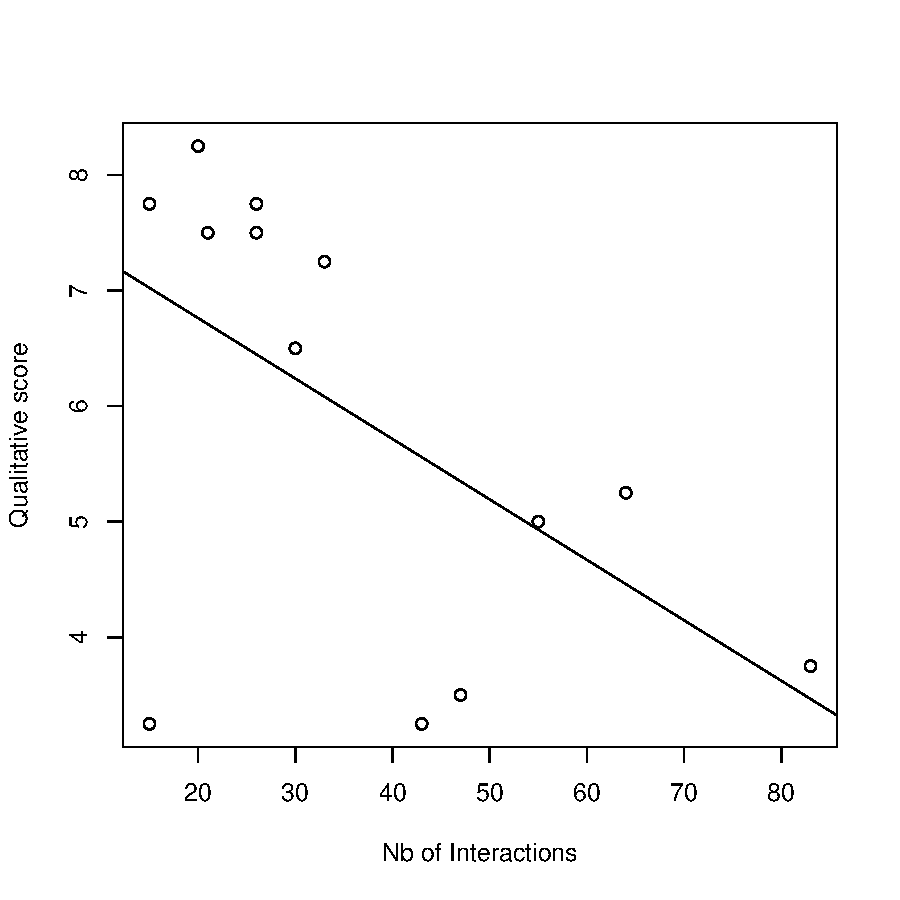
\includegraphics[width=\textwidth]{ranger-interactions-vs-qualitative-score}
%                \caption{Qualitative score by interactions}
%                \label{fig:qualitative-score}
%        \end{subfigure}
%        \caption{\textbf{The Ranger domino study: Child-robot interaction.}\\
%    \textbf{a)} Quantitative assessment: here, six interaction modalities have
%        been selected: showing something to the robot ({\tt show}), talking to
%        the robot ({\tt talk}), touching it ({\tt touch}), misbehaving (like
%        shaking it, {\tt mis}), using gestures ({\tt ges}), and looking
%        for help by glancing at the experimenter ({\tt look}). In each
%        of the 13 experimental runs, we annotated and counted the number of
%        occurrences of each of these interactions. Highlighted runs 2.3, 2.4,
%        2.7 and 2.8 correspond to unexpected robot behaviors: we observe peaks
%        of interactions every time the robot's behavior changes from expected to
%        unexpected or from unexpected to expected. (n = 26 children)\\
%	\textbf{b)} We found a significant negative correlation ($p=0.048$) between the
%    number of interactions and the qualitative anthropomorphic projections. This 
%    suggests that children who interacted more with the robot, anthropomorphized it 
%	less, and \textit{vice versa}. (n = 13 groups)}
%    		\label{fig:Ranger-domino}
%\end{figure}
%
%
%\subsubsection{Anthropomorphic interactions with the robot\\}
%
%The video recordings of the interaction session in which the children 
%played domino with the partly misbehaving robot were annotated according 
%to a coding scheme that we developed. Amongst others, six different types 
%of active actions / active engagement that a child carried out with the 
%robot were annotated. We understand some of these active engagement 
%actions as anthropomorphic, such as talking directly to the robot or 
%using gestures to the robot. The distribution of the interaction data per 
%run (see Figure \ref{fig:interactions-per-run} suggests that after the 
%robot started misbehaving (and thus became less predictable) children 
%tended to use slightly more active engagement interactions: gestures toward the 
%robot, and to talk more to the robot. Also, they were looking more often at the 
%experimenter, seeking help. 
%
%%\begin{figure}
%%    \centering
%%    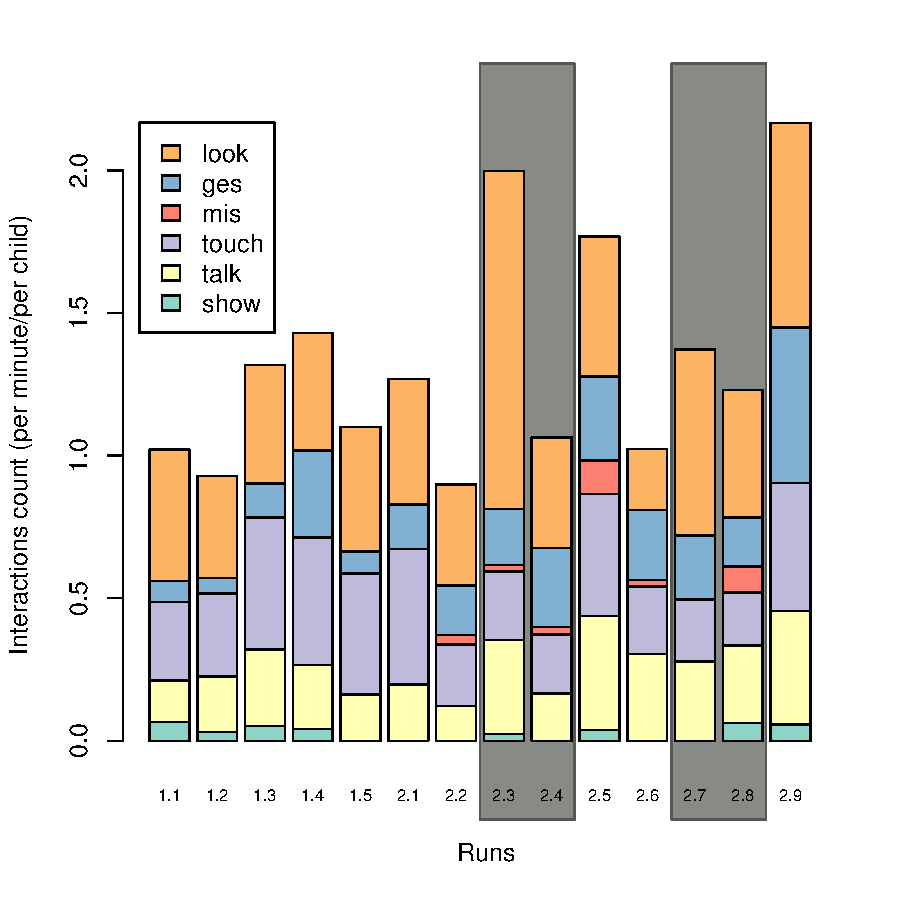
\includegraphics[width=0.5\columnwidth]{ranger-interactions-per-runs}
%%    \caption{Quantitative assessment: here, six interaction modalities have
%%        been selected: showing something to the robot ({\tt show}), talking to
%%        the robot ({\tt talk}), touching it ({\tt touch}), misbehaving (like
%%        shaking it, {\tt mis}), using gestures ({\tt ges}), and looking
%%        for help by glancing at the experimenter ({\tt look}). In each
%%        of the 13 experimental runs, we annotated and counted the number of
%%        occurrences of each of these interactions. Highlighted runs 2.3, 2.4,
%%        2.7 and 2.8 correspond to unexpected robot behaviors: we observe peaks
%%        of interactions every time the robot's behavior changes from expected to
%%        unexpected or from unexpected to expected. (n = 26 children)}
%%
%%    \label{fig:interactions-per-run}
%%\end{figure}
%
%
%\subsubsection{Perception of anthropomorphic characteristics of the robot\\}
%
%First of all, note that it is not at all easy to measure how far 4-5 year old's 
%perceive a robot to have some human-like qualities. We interviewed children about 
%various anthropomorphic traits of the robot, such as: Can the robot feel happy or 
%sad? Some of these questions were inspired by \cite{kahn_jr._robotic_2006}. For 
%each of these anthropomorphic traits questions, we gave a point if the child 
%answered in a positive way (partly reversed, negative way), indicating that the 
%child perceived the robot as somehow human-like. In the end, we summed up all 
%points, to obtain a \textit{qualitative score} for a child's tendency to 
%anthropomorphize the robot.
%
%
%\subsubsection{Summary Ranger domino study\\}
%
%We were trying to bring both measurements together: the anthropomorphic 
%interactions with the robot and the perception of anthropomorphic characteristics 
%of the robot. By this, we wanted to find out whether both aspects are correlated to 
%each other. A correlation would allow us to answer questions such as: Do children 
%that perceive more human-like characteristics in the robot also interact with it in 
%a more human-like way?
%
%
%%\begin{figure}
%%    \centering
%%    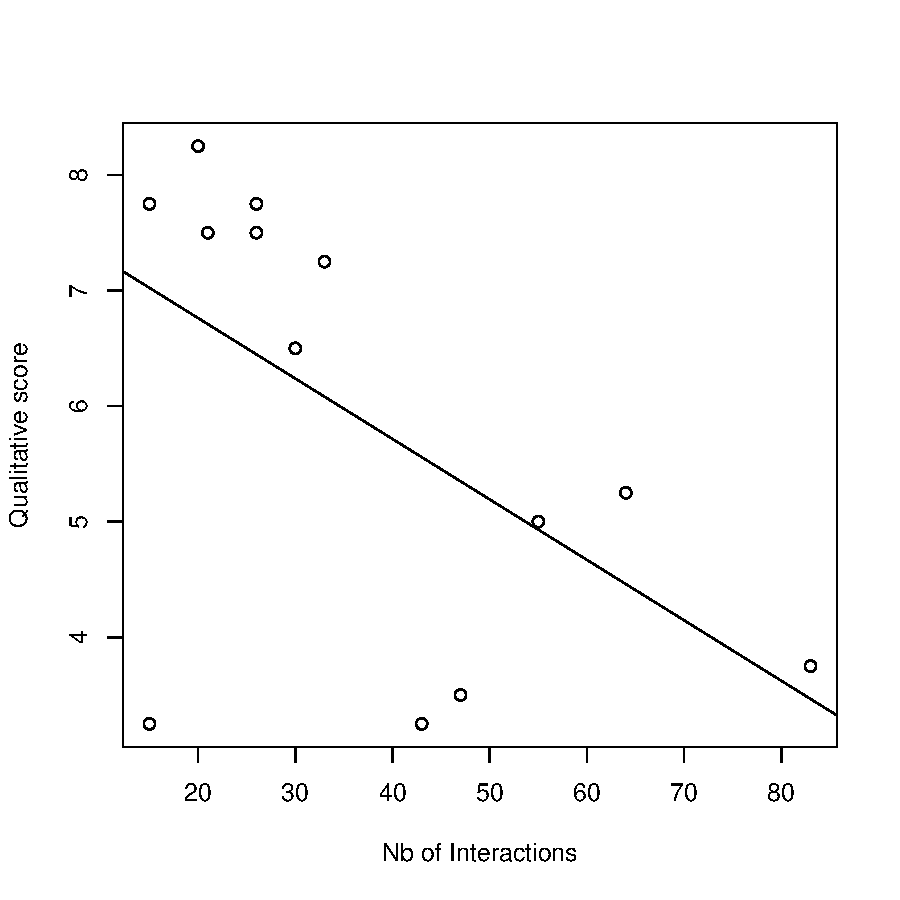
\includegraphics[width=0.5\columnwidth]{ranger-interactions-vs-qualitative-score}
%%    \caption{We found a significant negative correlation ($p=0.048$) between the
%%    number of interactions and the qualitative anthropomorphic projections. This 
%%    suggests that children who interacted more with the robot, anthropomorphized it 
%%    less, and \textit{vice versa}. (n = 13 groups)}
%%    \label{fig:qualitative-score}
%%\end{figure}
%
%Figure~\ref{fig:qualitative-score} plots the qualitative against the quantitative assessment of
%anthropomorphic effects during the Ranger domino study: the correlation is
%negative. This was a surprise. The more the children interacted with the robot, the less they
%projected anthropomorphic traits on the robot. We also note a remarkable cluster
%of seven groups of children who did not interact much with the robot, but had a
%strongly anthropomorphic perception of the robot. This may initially look
%counter-intuitive (one could hypothesize that the more playful the children are
%with the robot, the more likely they are to consider it as a friend/pet/lively
%being). We discuss possible cognitive explanations of this in Section~\ref{sec:cognition-neuroscience}.
%
%
%


%%%%%%%%%%%%%%%%%%%%%%%%%%%%%%%%%%%%%%%%%%%%%%%%%%%%%%%%%%%%%%%%%%%%%%%%%
%
%
%
%		PART 1: WHAT OTHERS DID AND WE ALREADY KNOW ABOUT ANTHROPOMORPHISM
%
%
%
%%%%%%%%%%%%%%%%%%%%%%%%%%%%%%%%%%%%%%%%%%%%%%%%%%%%%%%%%%%%%%%%%%%%%%%%%


\section{Anthropomorphism}
\label{sec:anthropomorphism}

Anthropomorphism is an interesting phenomenon because it tells us something about 
the relationship between the human who anthropomorphizes, and the non-human agent 
which is anthropomorphized. Though commonly observed, it still appears controversial, at 
the same time, that humans tend to \textit{``see human in the non-
human''} \citep{epley_seeing_2007}. 
To shed light on this phenomenon, first of all, we would like to propose a clarification of terms.
In short, we propose to differentiate between \textbf{anthropomorphic form} to refer to an imitation of human-like form in the \textit{design} of artificial agents, and  \textbf{anthropomorphism} to refer to the social phenomenon of 
people's tendency to \textit{perceive} human-likeness in non human-like agents.
\citep{fink_anthropomorphism_2012} In the following, we might use the terms \texit{form} and \textit{design} interchangeably.

As anthropomorphism arises in an interaction between a human and a non-human agent
\citep{persson_anthropomorphism_2000}, one can also
take two main perspectives on explaining anthropomorphism \citep{lee_human_2005}: an artifact-centered perspective and a human-centered perspective. 
We now first present an artifact-centered perspective, and outline how 
robotics uses \textit{anthropomorphic design} to encourage 
people to interact in a social, human-like way with robots.
Then, we present a human-centered 
perspective and shed light on \textit{anthropomorphism as a social phenomenon}. We present 
theories from psychology and cognitive science to explain people's tendency to 
perceive human-like characteristics in non-human agents.
It has to be kept in mind that both perspectives are inseparable; they apply at the 
same time, and we would like to present them here just as two different viewpoints 
on the same phenomenon.
In the end of this section, we synthesize 
the presented backgrounds into an extended understanding of anthropomorphism 
as a multi-factor phenomenon.


%%%%%%%%%%%%%%%%%%%%%%%%%%%%%%%%%%%%%%%%%%%%%%%%%%%%%%%%%%%%%%%%%%%%%%%%%
%
%
%
%		ARTIFACT-CENTERED PERSPECTIVE: ANTHROPOMORPHIC DESIGN
%
%
%
%%%%%%%%%%%%%%%%%%%%%%%%%%%%%%%%%%%%%%%%%%%%%%%%%%%%%%%%%%%%%%%%%%%%%%%%%	 

\subsection{An artifact-centered perspective on anthropomorphism}
\label{sec:anthropomorphic-design}

An artifact-centered perspective explains anthropomorphism from the ascertainable 
parts of the non-human agent, namely the anthropomorphic form of it.
Using the term \textit{form} to describe the design of an artifact, we refer 
not only to the shape (how it looks like) but to the total 
expression of the artifact \citep{bartneck_shaping_2004}. \cite{disalvo_hug:_2003} 
argues that \textit{form} includes a product's physical shape, materials, and 
behavioral qualities. The behavioral aspect is of special importance for interactive 
systems that show some degree of autonomy (independence).
Several categories of anthropomorphic form can be classified, but there is no 
common agreement on the borders and transitions between these categories: 
anthropomorphic, zoomorphic, caricatured, functional \citep{fong_survey_2003}.
The use of nature-inspired and in particular anthropomorphic (human-like) form in the 
design of non-human things is as old and manifold as people's tendency to anthropomorphize. 
Anthropomorphic (and life-like) forms have a long-standing tradition in design in general, and in the design of daily life things, in particular 
\citep{norman_design_1988,guthrie_bottles_2000}. Interestingly, from its very beginning robots were resembling a human being in their appearance. Starting from when the term \texit{robot} first appeared in a play by Karel \^{C}apek in the 1920ies, robots were man-made beings, created as the \textit{``shadow of man''} \citep{replicant_????}.

The direction of causality in the artifact-centered view is that the non-human artifact 
(or a certain feature of it) encourages the human to anthropomorphize it. 
This perspective assumes that humans directly (mindlessly) respond to life-like and social 
cues that the non-human agent or system emits \citep{nass_machines_2000}. Without thoughtful mental processing, 
humans tend to simply apply stereotypes and heuristics to the non-human agent, and in turn apply human-human social schemas and norms to the occurring interactions.
\cite{takayama_perspectives_2012} propose to refer to this immediate (sometimes visceral) sense in a situation as \textit{in-the-moment}, compared to a more distanced cogitation and consideration which she calls \textit{reflective}. (As this distinction imply different cognitive processes, we will come back to it later, in the human-centered perspective, Section \ref{sec:human-centered}). 

The view of people mindlessly reacting in a human-social manner to anthropomorphic forms
is based on the fact that humans naturally react to specific 
cues. From early childhood 
on, humans are inherently well-trained to perceive life \citep{epley_seeing_2007}, 
or to respond to social cues, such as facial expressions, social gestures or turn-taking. Humans have a propensity toward particular cues that seem to trigger automatic interpersonal social responses \citep{takayama_perspectives_2012}. 
One has to keep in mind that in 
human-human interaction these cues are of various senses and modalities, 
and consequently human-like design is also realized addressing several senses. 
One of the most outstanding aspects is probably the outer appearance of an agent or 
artifact (in particular when it is unknown or unfamiliar). \cite{schmitz_concepts_2011} 
argues that an agent's outer appearance is likely to have an important impact on how 
the object is overall perceived. Consequently, if a robot's outer form resembles a 
human, the robot is likely to be treated similar to a human. Besides the physical shape of a robot, other more subtle anthropomorphic forms can be found in robots, including human-social behavioral cues (\eg eye-gaze), social gestures (\eg waving), or verbal politeness (\eg greeting, apologizing).

People's natural reaction to these and other anthropomorphic design cues of
robots (in particular, social or also called \textit{sociable} robots 
\citep{breazeal_sociable_2000}) are extensively studied. This research is of particular interest in human-robot interaction as the consequences of anthropomorphic design can be both of positive and negative nature, and it is yet not clear what exactly it is that makes the difference.


\subsubsection{How people perceive and interact with human-like robots\\}
\label{sec:anthropomorphism-robotics}  
 
Most work that studies how far human users treat robots as social agents, builds on the 
famous work of \cite{reeves_media_1996} in HCI. In the so-called \textit{Media 
Equation}, the authors describe that people mindlessly react in a social way to their computer 
and that they tend to even attribute human (social) characteristics to it -- despite 
the fact that a computer does not have human-like characteristics. Apart from 
computers, anthropomorphism has also been observed with digital / virtual characters 
\citep{von_der_putten_it_2010}, and artificial embodied agents, 
such as robots \citep{rosenthal-vonderputten_experimental_2013}. 
In short, one can say that with robots, and human-like robots in 
particular, anthropomorphism is a commonly observed phenomenon. 
But what are the motivations which underlie the efforts of enhancing anthropomorphism 
through specific anthropomorphic design in robots? Why are anthropomorphic forms so 
distinct and at the same time controversial in robotics? There is no one single answer 
to these questions. 
 
The underlying central point about the human-like design of robots lies in the 
implications that this design holds, and the suggestions for interactions that
it makes to the human user. 
In other words, the appearance 
and function of a product, whether it is an appliance or a humanoid robot, affects how 
people perceive it, interact with it, and build long-term relationships with 
it \citep{bartneck_shaping_2004}. 
The principle of human-like form is probably most prominent in the design of robots, 
due to several reasons, such as to foster efficient interaction and increase 
acceptance. An anthropomorphic design of a robot encourages people to reason about this 
unfamiliar system \emph{as if} it was a human. To increase this tendency, robots are 
designed with anthropomorphic (or lifelike) forms, or are able to display and use 
human-social cues when interacting with humans.
However, anthropomorphic robot designs have been controversially discussed and received 
remarkable attention since the early 1970ies, related to \cite{mori_uncanny_1970} 
theory of the \textit{Uncanny Valley}, see Figure \ref{fig:uncanny_valley}.

\begin{figure}\centering
% Use the relevant command to insert your figure file.
% For example, with the graphicx package use
  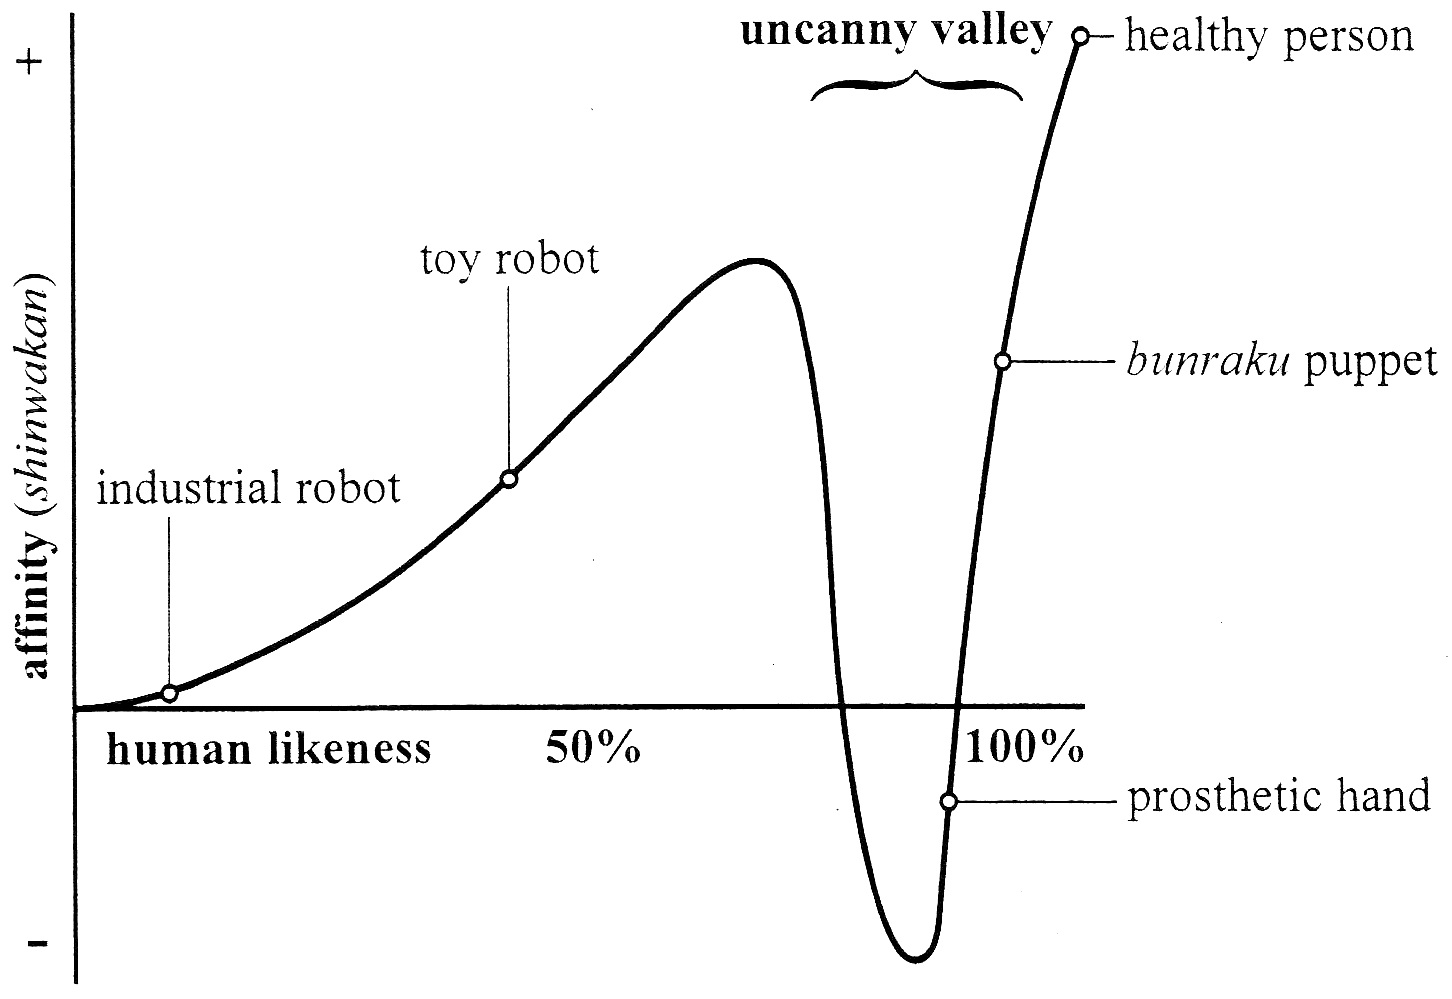
\includegraphics[scale=0.75]{uncanny-valley.jpg}
% figure caption is below the figure
 \caption{Mashiro Mori, illustration of the \textit{Uncanny Valley} hypothesis. The curve models the user's perceived affinity with the artifact, as its human likeness is increased. Up to a certain (not yet defined) point, a person perceives more affinity in a more human-like agent; however with an abrupt shift towards a negative perception as soon as the agent surpasses this point, of resembling a human too closely but not fully. Originally from 1970; picture from a manuscript version of \cite{mori_uncanny_2012}}
 \label{fig:uncanny_valley}       % Give a unique label
 \end{figure}

Despite the fact that the Uncanny Valley theory was more a working hypothesis and not 
meant to be empirically examined \citep{cheetham_human_2011}, it has been studied quite 
extensively. However, results are inconsistent. We try to give a short overview (not 
exclusive) on work related to HRI and robotics in the following. 
 
 
\subsubsection{Anthropomorphic form can be advantageous for HRI\\}

On one hand, developers and designers have discovered that human-like robots may better 
match the affordances that this to humans adapted world brings along. 
Apart from this, it is suggested that an increased human-likeness of a robot (up to a 
certain threshold) will generally lead to 
more perceived \textit{affinity} from the human side \citep{mori_uncanny_1970} (see 
Figure \ref{fig:uncanny_valley}).
This further increases anthropomorphism, and as such
appears to be beneficial for human-robot relations, especially with socially 
interactive robots \citep{fong_survey_2003}. Consequently, the domain of (social) 
robotics tries to exploit this by using
anthropomorphic forms in robots.
Humans seem to readily accept and prefer the 
anthropomorphic form of a robot (up to a certain point), when compared to purely mechanical 
robots. A possible explanation for this is that perceiving a system as
human-like (or also pet-like) compared to machine-like changes the 
way how users try to understand and make sense of this system. The reason for this is 
that humans tend to project everyday 
\hl{expectations} of human and animalistic life onto artificial agents that use 
anthropomorphic (or zoomorphic) forms \citep{schmitz_concepts_2011}. 
Both cognitive science 
and social psychology can provide explanations for this process of projection. The basic idea 
is that \textit{"the more similar in 
appearance, the more people are likely to use themselves as a source of induction 
and anthropomorphize these nonhuman agents"} \citep{epley_seeing_2007}. Studies have further 
shown that perceived similarity between the user and the robot influences the intensity of 
the participants' attributions towards the robot. Thus, the anthropomorphic design of a robot 
impacts the user's perception of the robot, and how far the user is likely to attribute and 
experience qualities such as intelligence, fun, or intentions in the robot. 
These experiences mark the transition between an immediate \textit{in-the-moment} and more thoughtful \textit{reflective} \citep{takayama_perspectives_2012} perception of, and interaction with the robot. As such, a more human-centered perspective needs to be applied, and we will come back to this in Section \ref{sec:human-centered}.

In short, the central point in using anthropomorphic design in sociable robots is that 
humans tend to apply the same communication references to anthropomorphic robots 
that they would use with other humans, which in turn enhances feeling familiar and 
comfortable when interacting with the otherwise unknown system.
This positive effect has been shown in various 
empirical studies. It has been found that robots with human-like forms can enhance social 
responses from humans which in turn can positively impact on acceptance 
\citep{duffy_anthropomorphism_2003,goetz_cooperation_2002,venkatesh_theoretical_2000}. 
People responded more positively to an artifact that displayed human-like 
behavioral characteristics (emotions, facial expression) in contrast to a purely 
functional design 
\citep{eyssel_anthropomorphic_2010,krach_can_2008,reeves_media_1996,riek_how_2009}. 
Overall, these results suggest that human-like features in robots enhance 
anthropomorphism, and in turn create a social view toward the robot.

 
%Anthropomorphism represents just one of many examples of induction whereby "people reason about an unknown stimulus based on a better-known representation of a related stimulus" \cite{epley_when_2008}, in this case reasoning about a non-human agent based on representation of the self or other humans.


\subsubsection{Anthropomorphic form can be disadvantageous for HRI\\}

The anthropomorphic form also 
increases people's expectations of the agent, and consequently, a very human-like 
appearing robot is not only perceived but also expected to act like a human. However, today's artificial systems are 
not able (yet) to mimic well human movements, or human social cues in an acceptable way. 
The case is that the artificial agent pretends to be human but fails, and this is 
more than just disappointing for the 
human -- it appears uncanny and evokes reluctance, the so-called 
\textit{"uncanny valley"}. The idea of naming this shift and drop from a positive to a negative reaction,
follows Freud's description of the so-called \textit{uncanny} (a translation from the German word 
\textit{``unheimlich''}). Controversially, something uncanny \textit{"derives its terror not from 
something externally alien or unknown but -- on the contrary -- from something 
strangely familiar which defeats our efforts to separate ourselves from it"} (v. Foerster, cited after \cite{hegel_understanding_2008}).
In other words, humans are very sensitive to the limits of what is familiar to them 
in a sense of being human. At the same time, humans are naturally very skilled when 
it comes to identifying what is acceptable as a human and what is an imitation 
of it. Even subtle differences can be crucial -- humans are inherently well trained 
in identifying if there is \hl{``something strange''} in the familiar.
Summing it up, a not yet very well defined thin line separates acceptable human-like forms in 
robots from creepy artificial \textit{almost} human-like appearing robots.

 
Of course, there is no one good answer to the question how to not fall in the 
uncanny valley when designing an anthropomorphic system. Equipping a system with 
some anthropomorphic forms seems to be inevitable 
\cite{duffy_anthropomorphism_2002} in the advancement of human-machine interfaces 
and sociable robots \citep{breazeal_sociable_2000}. However, we agree that 
\textit{"the important criterion is to seek a balance between people's expectations 
and the machines capabilities"} \citep{duffy_anthropomorphism_2002}. 





% Simulation Theory

%Findings that support anthropomorphic form in robots because they found people 
%respond with anthropomorphizing these kind of robots, and in turn act more social 
%toward them or accept them more easily:	empathy --> check Iolanda's paper


%For instance, recent studies found that people tend to ascribe personality and 
%intentions to robots \hl{(REFS)} and that they show empathetic behavior toward robots 
%\citep{rosenthal-vonderputten_experimental_2013}. 

%Various studies have shown that people directly talk to their robot (even if it 
%does not recognize speech), give it a name, greet it, or wonder about its 
%intentions and actions as if it were a human 
%\citep{eyssel_anthropomorphic_2010,fink_anthropomorphic_2012,forlizzi_how_2007,fussell_how_2008,kiesler_anthropomorphic_2008}.
%It has frequently been described that people ascribe intentions or emotions to 
%their domestic robot, such as to a Roomba vacuum-cleaning robot 
%\citep{krumm_my_2007,sung_robots_2009} or the AIBO robotic dog 
%\citep{friedman_hardware_2003}.



%%%%%%%%%%%%%%%%%%%%%%%%%%%%%%%%%%%%%%%%%%%%%%%%%%%%%%%%%%%%%%%%%%%%%%%%%
%
%
%
%		HUMAN-CENTERED PERSPECTIVE: SOCIAL PHENOMENON
%
%
%
%%%%%%%%%%%%%%%%%%%%%%%%%%%%%%%%%%%%%%%%%%%%%%%%%%%%%%%%%%%%%%%%%%%%%%%%%	

\subsection{A human-centered perspective on anthropomorphism}
\label{sec:human-centered}

In contrast to the artifact-centered perspective, in the human-centered perspective the argumentation is, that the human is motivated to anthropomorphize the non-human artifact). As already mentioned, both these views go hand in hand.

Humans tend to perceive human-like characteristics such as physical appearance, emotional states, or inner mental states and motivations in non-human agents that do not have these characteristics themselves, such as animals, natural forces, religious agents, technological gadgets, or mechanical devices \citep{epley_when_2008}.\footnote{According to \cite{epley_when_2008}, a non-human agent can be anything that acts -- or is believed to act -- with apparent independence.}  Anthropomorphism has received remarkable attention across various different domains, such as natural sciences, developmental and social psychology, Human-Computer Interaction (HCI), and Human-Robot Interaction (HRI).

Originally, the term \textbf{anthropomorphism} comes from the Greek \textit{`anthropos'} for `man' (or `human') and \textit{`morphe'} for `form / structure' (or `shape'). Anthropomorphism is generally understood as people's tendency to perceive a non-human agent as if it had some human characteristics or traits. In turn, how a person perceives an agent further determines how she relates to and behaves towards the agent, or how she may behave in light of this agent \citep{epley_when_2008}.
As such, anthropomorphism can be seen as a special kind of relationship between a human interacting with a non-human agent. This anthropomorphic relationship is often characterized by the fact that the human attributes human-unique characteristics to the non-human agent. Since anthropomorphism becomes observable through these attributions, some definitions claim that anthropomorphism is not the perception but rather the attribution of human attributes to non-human agents, and name thoughts, emotions, and intentions as examples. The most prominently anthropomorphized non-human agents are probably animals and robots \citep{duffy_anthropomorphism_2003,schmitz_concepts_2011}.

Apart from anthropomorphism there also exists the term \textbf{animism}, which can be defined as the attribution of life to the nonliving. The study of animism was pioneered by Piaget in the 1920s with his work on \textit{The Child's Conception of the  World}. He found that children tend to regard many inanimate objects as capable of sensations, emotions and intentions, and called this view `animism'. Since then, children's inferences about the world have been studied intensively. However, there is an agreement that children's views and concepts of living, animal, and plant evolve as they grow up. Using this definition, animism differs in two main aspects from anthropomorphism:
First, the property which is ascribed differs: life-likeness is not human-unique but applies to all living beings. The second difference between anthropomorphism and animism stems from the agent (or better artifact) to which life is attributed. Living beings (most importantly animals) are naturally excluded from being animized. Consequently, while animals can be anthropomorphized (perceived to have human unique characteristics), they cannot be animized as they are already living beings. (Similarly to the fact that humans cannot be anthropomorphized as they are already humans.)
Often synonymously used to animism is the term \textbf{zoomorphism}, which applies to the cases when non-lifelike instances / things are associated with animalistic attributes, excluding human-specific traits. Both anthropomorphism and animism / zoomorphism can be embraced by the concept of \textbf{life-likeness}.

To illustrate better how anthropomorphism differs from attributions of animacy or life-
likeness, it is worth looking at paraphrases and examples of it. That is to say, 
anthropomorphism can alternatively be understood as \textbf{humanization} or 
\textbf{personification} of anything other than a human being. Personification has 
ancient roots, \eg in mythology but also in storytelling. For instance, anthropomorphism was also 
used to describe and be able to predict natural forces or anticipate great spirits.

There exists also the inverse phenomenon to anthropomorphism, which can be found in the literature as \textbf{dehumanization} \citep{haslam_dehumanization:_2006}, or \textbf{mechanomorphism} \citep{caporael_anthropomorphism_1986}. We do not treat this here.

% \begin{figure}[b]\centering
%% Use the relevant command to insert your figure file.
%% For example, with the graphicx package use
%  
\includegraphics[scale=1]{north-wind.jpg}
%  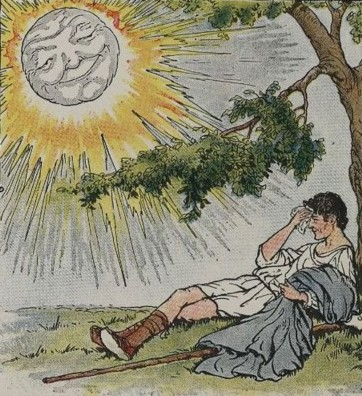
\includegraphics[scale=1]{sun.jpg}
%% figure caption is below the figure
% \caption{Milo Winter illustration of Aesop Fable \textit{The North Wind and the Sun}, 1919; both natural forces wind and sun are anthropomorphized with a human face; picture source: wikipedia}
% \label{fig:north-wind-sun}       % Give a unique label
% \end{figure}


%An illustration of an anthropomorphism related to nature is shown in Figure 
%\ref{fig:north-wind-sun}. In this Milo Winter (1919) drawing \textit{"The North Wind 
%and the Sun"}, both north wind and sun are given a human face.


\subsubsection{Why do people anthropomorphize?\\}
\label{sec:explanations}

But why do people anthropomorphize? First and foremost, it needs to be mentioned that anthropomorphism is a fairly complex phenomenon. Paradoxically, there is a huge and diverse body of literature on it but nevertheless, it seems that anthropomorphism is still not very well understood (especially in a field as young as HRI).

One common reason for anthropomorphism is that by perceiving some human-like characteristics in the non-human agent, this agent is made more \emph{graspable}, \emph{understandable}, \emph{predictable}, and one can feel \emph{more empathetic} toward it, and possibly one can then anticipate the agent's behavior. These are central motivations when trying to explain anthropomorphism, and we will come back to them in more detail later on. 
It is described that for the just mentioned reasons, people commonly anthropomorphize their pets, by ascribing mental states, intentions or feelings to them\footnote{Interestingly, pet-ownership seems to have a significant impact on human-robot interaction: several studies suggest that pet-owners are more likely to anthropomorphize technologies and robots than non pet-owners} \cite{eddy_attribution_1993}. But how can these motivations behind anthropomorphism be explained from a human-centered point of view?

%Anthropomorphism as a social phenomenon arises in an interaction \citep{persson_anthropomorphism_2000}, and thus includes at least two interaction partners (the human and the real or imagined non-human agent). Therefore, one can take two main perspectives on explaining it \citep{lee_human_2005}: a human-centered, and an artifact-centered. We briefly outline both views in the following. It has to be kept in mind that both perspectives are inseparable; they apply at the same time, and we would like to present them here just as two different viewpoints on the same kind of phenomenon.


This perspective builds on research from developmental and social psychology as well as cognitive sciences.  In the following, we present what we found in reviewing this literature: (1) a line of research in developmental psychology that studies the attribution of animacy; (2) a line of research in more cognitive sciences that studies the cognitive processes that underlie anthropomorphism, and (3) a theory that explains anthropomorphism based on psychological factors~\citep{epley_seeing_2007}. All three branches apply a human-centered perspective on anthropomorphism.


\paragraph{Developmental psychology research on the attribution of animacy and intention\\}

The phenomenon of attributing animacy and intentions to nonliving objects such as simple shapes has been intensively studied in developmental psychology. As mentioned earlier, Piaget found that children tend to ascribe life to the nonliving. They also tend to interpret physical phenomena in terms of intention on the part of the non-human subject. For instance children are likely to argue that \textit{``the sun is hot because it wants to make people warm''} \citep{leeds_childrens_1992}. In this example it is in fact questionable whether children really anthropomorphize the sun (believing that it has an intention) or whether they are using anthropomorphism in a metaphoric sense (because their conceptions of the world and of the living are not yet fully formed). Later however, two famous experiments by \cite{heider_experimental_1944} and \cite{michotte_perception_1963} showed that also adult participants attribute animacy and intention to simple things and shapes based on motion.\footnote{For more details, the reader may refer to the ``attribution theory''.} In both experiments, participants viewed animations of simple shapes, such as circles or triangles. 
%(see Figure \ref{fig:animacy_attribution})
Asked to describe what they observed, most people developed elaborate stories, attributing motivations, emotions and relationships between the objects.

%\begin{figure}[h]\centering
%% Use the relevant command to insert your figure file.
%% For example, with the graphicx package use
%  
\includegraphics[scale=0.6]{heider-simmel_animation.jpeg}
%% figure caption is below the figure
% \caption{Fritz Heider and Mary-Ann Simmel's animated film to study people's tendency to attribute animacy and intention to simple shapes; \textit{An experimental study of apparent behavior}, 1944}
% \fxnote{wrap text around this figure?}
% \label{fig:animacy_attribution}       % Give a unique label
% \end{figure}

Summing it up, as mentioned earlier, it seems that there is a natural, relatively spontaneous reaction that accounts for people's tendency to attribute animacy and intention to moving shapes, even when there is no similarity of the shape to a human. This tendency to animize / anthropomorphize is already developed (and even more distinct) in infants and children. Thus besides the anthropomorphic cues emitted by the design of the artifact, also developmental stages, and people's natural reaction play a role how far we interpret movements / motions (as one of the most basic "lifelike" cues), for instance.


\paragraph{Cognitive science research, the mental model theory (Theory of Mind)
and neural correlates of anthropomorphism\\}

Anthropomorphism and similar phenomenons can also be understood as a thoughtful process of induction whereby \textit{``people reason about an unknown stimulus based on a better-known representation of a related stimulus"}~\citep{epley_when_2008}. In the case of anthropomorphism this means a person's reasoning about a non-human agent based on the representation of the self or other humans. A central construct of this perspective is the so-called \textit{mental model} that a person has (and builds) of the agents she is reasoning about and interacting with. The specific mental model we have about an artifact / agent basically explains (in our individual way to ourselves) how this artifact / agent works the way it does.
There are two central aspects here, when looking at the quote from \citep{epley_when_2008} above.\\
\textit{(1)} One assumption is that the user is not familiar with the other agent. This is basically true for all other agents (and entities) but oneself because we can only be our self. This view is also consistent with the \emph{familiarity thesis}~\citep{hegel_understanding_2008} which claims that we understand the world based upon a mental model of the world that we are most familiar with (our self). Thus, we can best use our self as source of induction when reasoning about other agents. However, in case we would like to understand the behavior of a spider, we would probably not use our mental model of a human (or our self) simply because we do not have many things in common with a spider. And this is the second central aspect here.\\
\textit{(2)} One other assumption is based on the anthropomorphic design of the other agent (see Section \ref{sec:anthropomorphic-design}): if the agent behaves (appears) much like a human being (\eg a robot that emits a human voice), people's mental model of the agent's behavior is likely to approach their mental model of humans (though the model may differ in some important aspects).

This cognitive viewpoint on anthropomorphism is important because people's estimation of an agent's knowledge model and its capabilities affects the way they relate to it. This holds important implications for the resulting interaction with the system, the user experience, and the acceptance. Previous research examined the validity of the mental model concept with various kinds of robots \citep{schmitz_concepts_2011,kiesler_mental_2002}. Findings suggest that people tend to hold richer mental models of anthropomorphic robots in contrast to mechanic ones \citep{kiesler_mental_2002}.\footnote{\hl{Later in this article, we may however come to question how far this result is based on expectations from the human user side, which are likely to be refined after continued interaction, and after the user gets acquainted with the robot's behavior.}} 
A similar finding is described in \cite{hegel_understanding_2008} and
\citet{krach_can_2008}. In a user study using functional magnetic resonnance
imagery (fMRI), the authors found that participants
implicitly attributed human-like qualities, such as mental states, to their
non-human interaction partner. Indeed, from an early age humans develop a
tendency to explain one's own and others'actions in terms of beliefs, desires
and goals,  called \textit{theory of mind}. The theory of mind allows the implicit attribution of
intentions and other mental states to others \citep{premack1978does, leslie_pretense_1987, Frith2003}.
\citet{hegel_understanding_2008} and \citet{krach_can_2008} finding was evident at the behavioral level
as well as on the neuro-physiological level: the more the human-likeness of the
artefactual partner increases, the more brain areas associated with theory of
mind  get activated
\citep{krach_can_2008}. \footnote{\hl{Ha! This says that anthropomorphism can also occur on a behavioral level, yes! :) so we should also measure anthropomorphism in the behavior.}} 
Implication of human brain area involved in the inference of others` mental
states has also been shown in response to viewing
non-anthropomorphic/non-humanoid robotic gadgets whose behavior
has been described as unpredictable -- but not in response to those whose
behavior was described as predictable -- a finding also found at the behavioral
level \citep{Waytz2010}.
Interestingly, the grey matter volume of a brain area related to theory of mind
has been correlated to individual's score of anthropomorphism
\citep{cullen2013individual}.

At lower, more automatic, level, robots have been shown to elicit resonance behaviors in the
human brain. Resonance behaviors \citep{Rizzolatti1999} are mechanisms by which the brain areas involved in the internal representations of an action, an emotion or a sensation are equally recruited during the perception of another individual performing the same action or experiencing the same emotion or sensation.  
The neurons showing resonant properties have been called mirror neurons and
have been found in a wide range of modalities (motor, emotional etc..)
\fixme{addref}. Seeing a robotic arm reaching for an object activates the motor mirror neurons the same way as for seeing a human arm reaching for the same object
\citep{Gazzola2007, oberman_eeg_2007}. However, a study of emotion perception
on a robotic face found reduced activity in emotional brain
area known to have mirror properties in response to the robotic face compared to
a human face \citep{Chaminade2010}. Nevertheless, these authors showed that when
the participants were explicitly instructed to pay attention to the robot's
emotional expression, motor mirror neurons get activated.
Interestingly, using electroencephalography,  it has also been shown that
emotional behavior elicited by a robot face influences the speed of human
responses as well as early brain processes the same way as emotional expression
of a human face did \citep{Dubal2010}.


%


In sum, this branch of research suggests that anthropomorphism implies that
people thoughtfully develop a mental model of agents in their environment and
that they make inferences about these agents based on what is familiar to them
-- themselves, humans and human behavior. This understanding builds on the
theory of mind,  a
person's ability to attribute mental states to oneself and others. 
%A theory of mind for other agents enables us to attribute intentionality to those agents \citep{leslie_pretense_1987,admoni_multi-category_2012}. 
We briefly reviewed  neuro-physiological evidence of a link between the tendency
to thoughtfully anthropomorphize and the engagement of brain processes involved
in the attribution of mental states to other humans. The human-likeness quality
of the artefactual agent seems to play a role in the involvement of theory of
mind but also the unpredictable feature of the agent behavior alone seems to be
sufficient. Low-level mechanisms of the brain that allow humans to map others`
motor behaviors into their own repertoire are equally elicited when perceiving a
robot's action. It is not yet clear whether humans are processing emotional
signals from a robot the same way as they do for human beings. 
%were recently demonstrated at the brain level~\citep{cullen2013individual}.


\paragraph{Social psychology research: a 3-factor theory of anthropomorphism\\}
\label{sec:psychological-factors}

Social psychology offers interesting theories that can be applied to understand people's motivation to anthropomorphize. Irrespective of the artifact's characteristics, several psychological determinants have been found to explain a person's tendency to anthropomorphize. \cite{epley_seeing_2007} present a ``3-factor theory'' of when people are likely to anthropomorphize based on psychological determinants. Namely, the theory suggests that some people are more likely to anthropomorphize when: 

\begin{enumerate}
	\item ~anthropocentric knowledge is accessible and applicable to the artifact (\textit{elicited agent knowledge}),
	\item ~they are motivated to explain and understand the behavior of other agents (\textit{effectance motivation}), and
	\item ~they have the desire for social contact and affiliation (\textit{social motivation}).
\end{enumerate}

The first factor (\textit{elicited agent knowledge}) is a \textbf{cognitive determinant of anthropomorphism} and based on the idea that a person builds a mental model (theory of mind) of the other agent. \cite{epley_seeing_2007} suggest that the process of making inferences about non-human agents is based on the activation of knowledge about humans (or the self). As mentioned before, when a person builds a mental model of the other (unfamiliar) agent, the question here is why does she draw on knowledge about other humans / herself and not on something else? One basic reasons for this is a person's physical constraints of being a human and nothing else. Consequently, one has no other experience than the self and in turn people tend to make inferences about others' mental states by relying inordinately on their own mental state. \footnote{Using one's own mental states and characteristics as a guide when reasoning about other humans is called ego-centrism. In contrast, when using self-knowledge (or knowledge about humans in general) when reasoning about non-human agents, this is called anthropomorphism. See \cite{epley_seeing_2007}} Also empirical findings suggest that knowledge about humans in general, or self-knowledge in particular, is likely to serve as a readily accessible base for induction when reasoning about non-human agents. This tendency is usually stronger in young children and decreases with cognitive development and the learning to distinguish the self from other humans, and non-human agents. 
	
Both the second factor \textit{effectance} and the third factor \textit{sociality} are \textbf{motivational determinants of anthropomorphism}. \textit{Effectance} is understood a person's motivation to interact effectively in one's environment. That means, a person is motivated to be able to understand, predict, and reduce uncertainty \footnote{\hl{(this feeds again our hypothesis that as soon as a robot is not uncertain anymore, there is no need to keep on anthropomorphizing it)}}\fxfatal{important! move/copy that to the 'model' section or discussion} about her environment and the agents that inhabit it. According to \cite{epley_seeing_2007}, \textit{effectance motivation} can lead to anthropomorphism, since anthropomorphism serves as one way to reduce uncertainty and to increase comprehension of events in one's environment. Again, also according this factor it can be argued that children are more likely to anthropomorphize than adults. As children are in their early stages of life, they are likely to feel more uncertain within their environment, and consequently tend to anthropomorphize more.

The third factor \textit{sociality} describes a person's motivation for social contact, social connection, and social approval from other agents. In lack of social connections to other humans (\etc friends, family, colleagues), a person is more likely to compensate these social connections by anthropomorphizing non-human agents. In other words \textit{"[...] those who are chronically lonely should be more likely to anthropomorphize nonhuman agents than those who are more chronically connected"} \citep{epley_seeing_2007}. Importantly for anthropomorphism, this social connection often appears to be satisfied by connections with \textit{"two of the most commonly anthropomorphized non-human agents, namely pets and religious agents"} \citep{epley_seeing_2007}. Thus, the motivation of being socially connected increases the tendency to anthropomorphize non-human agents because first sociality motivation increases the tendency to perceive human-like characteristics and traits even in non-human agents, and second it increases the tendency to search for sources of social connection in one's environment.


\subsubsection{Diverse understandings of anthropomorphism\\}

We have seen that literature on anthropomorphism is quite diverse. We would like to point out that there exist different understandings of what anthropomorphism is. 
One reason for this might be that anthropomorphism
is a concept that is studied in very different domains that might each
integrate diverse or even contradictory understandings, or simply refer to different things.
However, the conflict is, that despite the fact that there is no commonly accepted definition, the terms
\textit{anthropomorphism}, \textit{anthropomorphic} or \textit{human-like} are
often used as if their meanings were clear and agreed upon
\citep{persson_anthropomorphism_2000}. Duffy \cite{duffy_anthropomorphism_2002} and \cite{epley_when_2008}
argue that these terms might even be misused. For instance, some researchers refer to \textit{"the
robot's level of anthropomorphism"} \cite{bartneck_is_2007}, whereas others
disagree to such a statement because they argue that the system or artifact itself does not \textit{"contain anthropomorphism" per se} but only gives rise to the process of anthropomorphizing in a
given user and situation. Consequently, \cite{persson_anthropomorphism_2000} conclude that
anthropomorphism emerges in the \textit{interaction} between the technology and
the user, and has to be understood as such. 
We will come back to this view later, in the summary of this section (Subsection \ref{sec:multi-factors}). 

Another paradox is that, while human's tendency to anthropomorphize is commonly observed, it is 
at the same time still rather poorly understood
\cite{epley_seeing_2007}. The phenomenon itself has been found to be very complex though sometimes
subtle and as such hard to study \cite{epley_when_2008,duffy_anthropomorphism_2002}. Further, it is not clear how to operationalize anthropomorphism. We would like to discuss the challenges of studying and measuring anthropomorphism toward the end of this article, in Section \ref{sec:measuring}.

%Anthropomorphism is used in different senses throughout different disciplines 
%\citep{duffy_anthropomorphism_2003} which makes it difficult to synthesize findings. 
Depending on which understanding of anthropomorphism is applied, not everything 
colloquially labeled as \emph{anthropomorphism} really is anthropomorphism.
One practical example is that, it is not always clear whether a person (may it be an adult or 
a child) who gives and anthropomorphic response, believes that the other agent really 
thinks or acts like a human or whether she is using anthropomorphism in a metaphoric 
sense.\citep{leeds_childrens_1992}.
Thus, we need to be clear about what we mean by anthropomorphism. 

But how to clarify the understanding of anthropomorphism?
From a psychology point of view \cite{epley_when_2008} try to clarify anthropomorphism by explaining what it is \textit{not}, and we think this approach could also help researchers in HRI and robotics. \cite{epley_when_2008} list four effects that anthropomorphism does not include:
(1) First, anthropomorphism does not include behavioral descriptions of observable actions. Anthropomorphism requires going beyond what is directly observable.
(2) Second, anthropomorphism does not merely entail animism, as animate life is not a uniquely human-like characteristic.
(3) Third, anthropomorphism does not include any requirement of reasoned or reflective endorsement of an inference.\footnote{\hl{(the strength of anthropomorphic inferences can vary)}}
(4) Finally, anthropomorphism is not necessarily inaccurate. A psychological theory should take this (in)accuracy in anthropomorphism into account and predict variability in the tendency to perceive human-like traits in non-human agents.\footnote{For more details, the reader may refer to the original work \citep{epley_when_2008}.}

Similarly to the last point mentioned by \cite{epley_when_2008}, several researchers argue that there might not just be one single type of anthropomorphism but different levels or gradations. For instance, \cite{persson_anthropomorphism_2000} proposes to understand anthropomorphism as a multi-layered phenomenon, and suggests that it exists of different levels, namely primitive categorization, primitive psychology, folk-psychology, traits, social roles, and emotional anthropomorphism. Correspondingly, \cite{ruijten_introducing_2014} propose to understand anthropomorphism as a continuum ranging from low to high human likeness, and to measure it as such. 
  

%%%%%%%%%%%%%%%%%%%%%%%%%%%%%%%%%%%%%%%%%%%%%%%%%%%%%%%%%%%%%%%%%%%%%%%%%
%
%
%
%		ANTHROPOMORPHISM AS A MULTI-FACTOR PHENOMENON
%
%
%
%%%%%%%%%%%%%%%%%%%%%%%%%%%%%%%%%%%%%%%%%%%%%%%%%%%%%%%%%%%%%%%%%%%%%%%%%	 



\subsection{Summary: Anthropomorphism as a multi-factor phenomenon}
\label{sec:multi-factors}

To sum it up, while anthropomorphism is a commonly discussed and
studied trait of human-robot interaction, its the understanding 
does not seem to take into account the wide range of phenomena that it
encompasses. To date, the understanding of anthropomorphism in robotics considers  two main factors: the
characteristics of \textbf{1) the robot's design} (degree of human-likeness) and
the psychological determinants in \textbf{2) the human user} (see
\cite{epley_seeing_2007}). A lot of research has shown that both these factors can
promote or hinder anthropomorphism.

However, based on what we have just presented, we would like to make a note, that there are more than these two factors that impact on anthropomorphism.

Based on the understanding that anthropomorphism represents a specific type of \textit{experience} that arises in the
\textit{interaction} between a set of user expectations and external reality
\cite{persson_anthropomorphism_2000}, 
%(see Figure~\ref{fig:anthropomorphism_and_interaction})
we propose that
anthropomorphism is a multi-layered phenomenon which arises in different levels, and is likely to evolve with continued interaction.
%we suggest to understand anthropomorphism as a \emph{dynamic},
%\emph{context-dependent} process. To this end, we apply Persson \textit{et
%al.}'s six levels on anthropomorphism to HRI and introduce three
%\emph{interaction phases}. These interaction phases of anthropomorphism reflect
%also the results of a long-term study that we conducted in a real human
%environment and provide an account of the so-called \textit{novelty effect}.

To this end, we make the following two suggestions:

First, we propose to include two more main factors as determinants of anthropomorphism (besides the robot's design, and the human user's characteristics). Namely, these factors are \textbf{3) the context of use} (situation) and the fact of getting used to a system the more and longer one interacts with it, thus becoming familiar with the system over \textbf{4) time}. 

%\begin{figure}[ht!]\centering
%% Use the relevant command to insert your figure file.
%% For example, with the graphicx package use
%  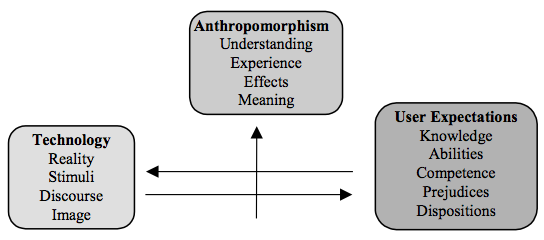
\includegraphics[scale=0.42]{persson_anthropomorphism.png}
%% figure caption is below the figure
% \caption{Anthropomorphism emerges in the (real or imagined) interaction between
% robot and user; illustration taken from \cite{persson_anthropomorphism_2000}
% \hl{maybe we don't put the figure here, it was just to illustrate what I mean}}
%
% \label{fig:anthropomorphism_and_interaction}       % Give a unique label
% \end{figure}

Second, we would like to take up the proposition already made by other researchers (\eg \cite{persson_anthropomorphism_2000,ruijten_introducing_2014}) to not viewing anthropomorphism as being either there or not there, but to discriminate different levels of
anthropomorphism (low, and high anthropomorphism, for instance).
This seems to make sense, since each of the four proposed factors has its own characteristics and involves specific
types of user expectations, for instance. Such a differentiation in the understanding of anthropomorphism could further allow to draw inferences
on the human-robot relationship based on the observed level of anthropomorphism.

\begin{figure}
    \centering
    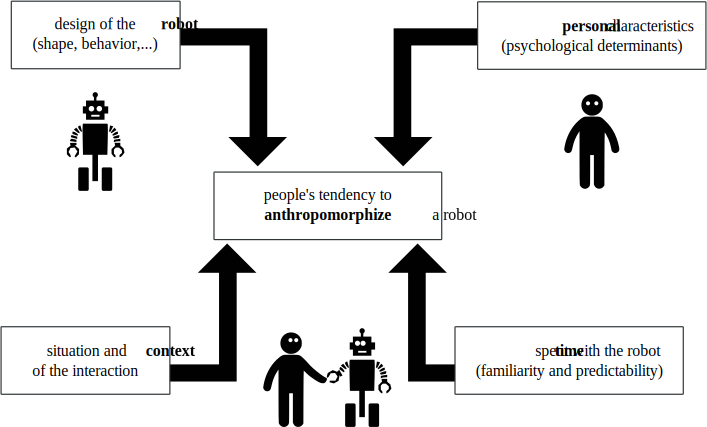
\includegraphics[width=0.7\columnwidth]{factors}
    \caption{Anthropomorphism is a multi-factor phenomenon. How far people tend to anthropomorphize a robot is determined by four main factors: the design of the robot $(R)$, the personal characteristics of the human user $(H)$, the situation and context in which the interaction occurs $(C)$, and the amount of time (repeated interaction) that the user spends to familiarize herself with the robot $(t)$.}
    \label{factors}
\end{figure}

To facilitate things, we introduce the notation \Ant[R,H,C,t] to reflect these multiple factors: we suggest here that
anthropomorphism is a function of a vector of robot's traits $R = \{r_0,...,r_n\}$, a vector human
determinants $H = \{h_0,...,h_n\}$, a set of interaction situations that build
an interaction context $C = \{s_0,...,s_n\}$, and the duration of the
interaction itself, $t$.

%% -> Commented out the overview as it does not match what we actually present... maybe we need a new one?
% We would further like to review and discuss research on anthropomorphism in
% robotics and human-like design of robots. We first provide a comprehensive
% understanding of the phenomenon drawing on theories from developmental
% psychology and cognitive sciences. We then present the trends of different
% kinds of anthropomorphic forms in robots and discuss their role in social
% robotics. The article integrates related work from human-robot interaction
% studies, reporting on findings from experiments with human subjects
% interacting with and evaluating various types of systems. We try to give a
% coherent view on the topic, outline similarities and antithetic findings, and
% contribute to a better understanding of anthropomorphism in robotics, and the
% acceptance of human-like characteristics in robots. We also aim to
% constructively discuss anthropomorphic design of personal and socially
% interactive robots. 

%In this article we will use the term \emph{anthropomorphic effect} to denote
%observable correlates of anthropomorphism. With these we include, amongst
%others, verbal utterances (such as direct speech or the use of pronouns
%"he/she"), (social) gestures (such as a hug, waving, deictic gestures) or
%\hl{anticipation of certain actions of an agent [what??]}.

% Persson \textit{et al.}
%suggest that the social phenomenon involves several levels, like primitive
%psychology, folk-psychology, social stereotypes, and emotional anthropomorphism. 



%%%%%%%%%%%%%%%%%%%%%%%%%%%%%%%%%%%%%%%%%%%%%%%%%%%%%%%%%%%%%%%%%%%%%%%%%
%
%
%
%				PART 2: OUR IDEAS -- A DYNAMIC PHENOMENON
%
%
%
%%%%%%%%%%%%%%%%%%%%%%%%%%%%%%%%%%%%%%%%%%%%%%%%%%%%%%%%%%%%%%%%%%%%%%%%%
%
% SEVERIN & JULIA: there will be 2-3 subsections in which we present our ideas:
% 	1) anthropomorphism is a multi-factor phenomenon (the figure with the several factors)
%	2) anthropomorphism is dynamic (the dynamic curve model)
%
%

\section{Anthropomorphism: a dynamic phenomenon}
\label{sec:our-ideas}

Why do we think that anthropomorphic projections are likely to change over time
and with growing experience a person has with a robot? The underlying process in
anthropomorphism is understood as reasoning about and perceiving something
non-human, and unknown or unfamiliar based on one's representation of the
familiar and well-known concept of being human (or one-self). The basic
operations underlying inductive inference are the acquisition of knowledge, the
activation or elicitation of knowledge, and the application of activated
knowledge at the time of the judgment \citep{epley_when_2008}. According to Epley
\textit{et al.}, the application includes attempts to correct, adjust, or
integrate less accessible information into a more automatically activated
default representation. This process can be seen as a process of correction, and
thus, it is often insufficient leaving final judgments biased in the direction
of the initially activated representation. As a person's knowledge base changes
/ evolves constantly with newly acquired things, or growing experiences with a
robot, etc., it is likely that the "need to anthropomorphize" a robot decreases
over time. First, because of the evolved knowledge about it, and second because
one has familiarized oneself with it. Consequently, the robot should become more
predictable and more familiar to the human user and inferences about it can be
made based on the acquired knowledge.  /fxfatal{confusing paragraph...needs
reformulation. Could also be turned into a section introduction instead of a
subsection}


So far, the HRI community has not much investigated how anthropomorphism in
human-robot interactions evolves over time (during the process of
\emph{adopting} a robot, for instance): we propose to go beyond the traditional
perception of anthropomorphism in robotics as a static feature that once
observed during a short-term interaction reflects a sustaining social effect.
Based on an extensive literature review previously
published~\citep{fink_anthropomorphism_2012} and field
experiments~\fixme{cites!}, we believe that anthropomorphic effects in HRI are
not always the same but evolve over time, along with growing interaction and
experience with the robot, similar to how relationships among people evolve
over time \fixme{(cite Hinde, 1988)}. In fact, \citet{kanda_interactive_2004}
also hypothesized that people's attitude toward technological artifacts and
their relationship with them would evolve over time, and they were among the
first who described \emph{novelty effects} during a long-term study with an
interactive robot in a school.


\hl{Julia: I need to work on this next paragraph but I would like to keep it here as a note}

\textbf{In-the-moment vs. reflective perspectives on agency}\\
Perception of agency can be treated as anthropomorphism.
\citep{takayama_perspectives_2012} proposes to differentiate between a \textit{in-the-moment} and \textit{reflective} perspective to better understand how human users perceive agency in robots.\footnote{``The other important distinction between the two perspectives is the \hl{cognitive processes} that they engage.''} According to Takayama, an \textit{in-the-moment} perspective refers to one's most immediate (sometimes visceral) sense in a situation. In contrast, a \textit{reflective} perspective refers to one's sense of a situation upon more distanced cogitation and consideration. For instance, we reflectively might not perceive agency in a social robot, but it can feel quite differently in the moment of interaction. A critical dimension of agency is the perspective from which something seems to have agency. \cite{takayama_perspectives_2012} argues that neglecting to separate reflective perspectives from in-the-moment perspectives of agency is one of the major sources of confusion when people talk and write about anthropomorphism. There seems to be a disconnection between what people consciously perceive and how they respond to stimuli that they may not consciously perceive.
That means, in the initial phase of interacting with a novel device \textbf{(initialization)} people might not consciously respond but rather mindlessly \citep{nass_machines_2000}. Only after some time of \textbf{familiarization}, they might respond in a more reflective manner. This can be illustrated by the fact that people tend to deny interacting with computational systems as if they were people and yet they respond to computers in many ways that are remarkably similar to how they respond to people \citep{reeves_media_1996}.
\cite{takayama_perspectives_2012} also applies a cognitive viewpoint on the two different perspectives of in-the-moment \vs reflective to illustrate differences. She states that in-the-moment perceptions of agency are largely shaped by bottom-up perceptual processes, evoking very immediate responses (\eg to the cues emitted by the artifact's design, see Section \ref{sec:anthropomorphic-design}).
In contrast, according to Takayama, reflective perceptions are more often shaped by top-down processes because of the nature of reflective thought.



\subsection{A Model of the Dynamics of Anthropomorphism}
\label{sec:dynamics-model}

The phenomenological model of anthropomorphism we propose
(Figure~\ref{fig:dynamics}~\citep{lemaignan2014dynamics}) represents how the
level of anthropomorphic effects~\Ant[R,H,C,t] (\ie observable manifestations of
anthropomorphism, as defined in section~\ref{sec:intro}) evolves over a
long-term human-robot interaction.

While the model primarily considers \emph{long-term interaction} -- direct
(non-mediated), repeated interaction with the same robot, over an extended
period of time (typically longer than a week), we also formally introduce a
so-called \emph{novelty effect}~\citep{kanda_interactive_2004} that models the
first phase of human-robot interaction, during which a specific increase of
anthropomorphic interactions is observed.

In this model, anthropomorphism is quantified by a \emph{normalized level of
anthropomorphic effects} $\antNorm[R,H,C,t] = \frac{\ant[R,H,C,t]}{\antMax}$: because anthropomorphic effects are
not quantified on an absolute scale, we present them as a normalized value, that
spans from a minimum (no anthropomorphic effects: $\ant=0$) to a maximum (noted
\AntMax, with $t_{max} = \operatorname{arg\,max}_t \, \ant[t]$). For readability
reasons, we however omit the hat on \Ant in the following sections. We discuss
at section~\ref{measuring} possible methodologies for the quantitative and
qualitative assessment of anthropomorphic effects.

As pictured on Figure~\ref{fig:dynamics}, we suggest that $t_{max}$ actually
corresponds to the novelty effect peak. The actual maximum value of
anthropomorphic effects depends on each unique combination of human, robot and
several other factors we introduce below, and thus varies. The general
\emph{shape} of the model remains however the same and depicts the evolution of
anthropomorphism over time, \ie the general dynamics of anthropomorphism.

The model takes into account the duration of the interaction, the nature of the
interaction, as well as acquired experience and familiarization mechanisms. We
also formally introduce a so-called \emph{novelty effect} that models the first
phase of human-robot interaction, during which a specific increase of
anthropomorphic interactions is observed. We focus on \emph{long-term
interaction}, \ie direct (non-mediated), repeated interaction with the same
robot, over an extended period of time (typically longer than a week). The nature 
of the interaction (goal-directed, entertainment, etc.) may
however vary.


\begin{figure*}[htb]
\centering


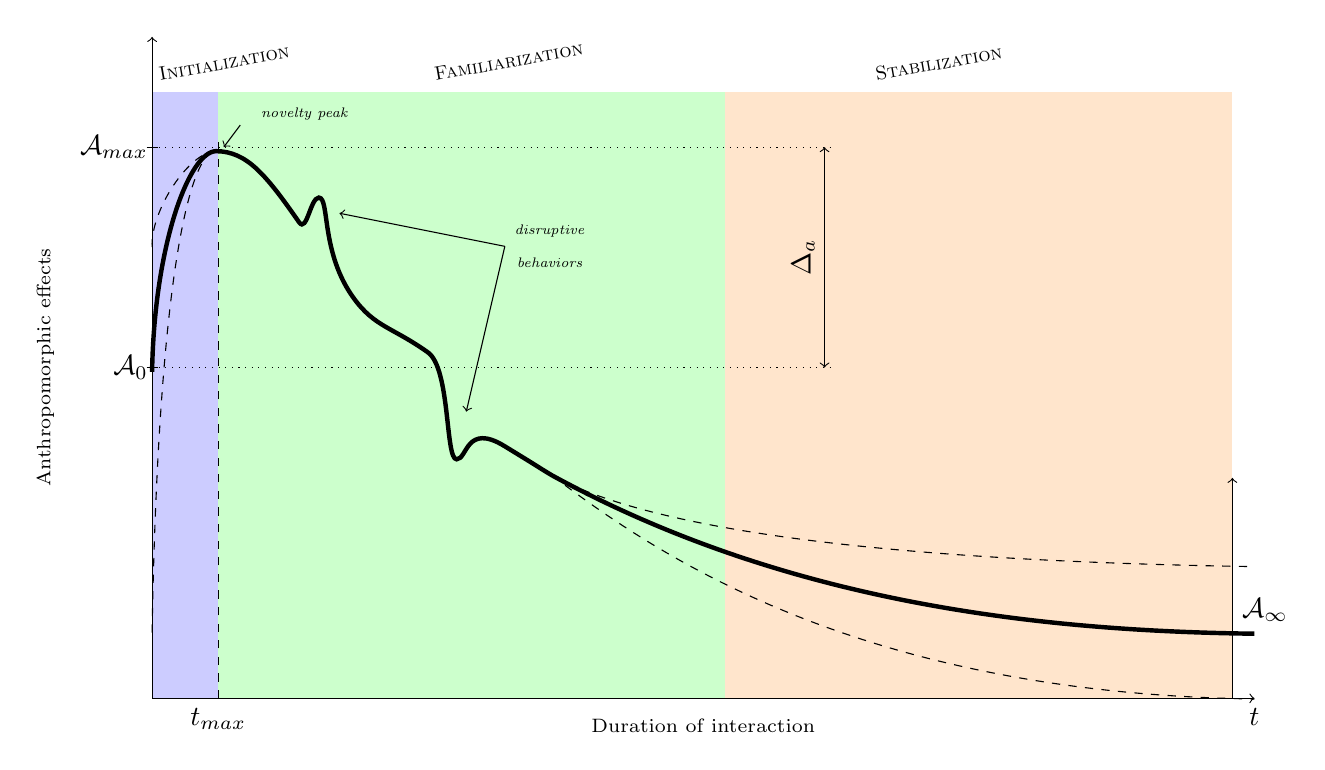
\begin{tikzpicture}[scale=1.4]

% background shading
\path[fill=blue!20] (0,0) rectangle (0.6,5.5);
\path[fill=green!20] (0.6,0) rectangle (5.2,5.5);
\path[fill=orange!20] (5.2,0) rectangle (9.8,5.5);
\draw(0,5.5) node[anchor=south west, rotate=10] {\scriptsize \sc Initialization};
\draw(2.5,5.5) node[anchor=south west, rotate=10] {\scriptsize \sc Familiarization};
\draw(6.5,5.5) node[anchor=south west, rotate=10] {\scriptsize \sc Stabilization};
% horizontal axis
\draw[->] (0,0) -- (10,0) node[anchor=north] {$t$};
\draw(5,-0.1) node[anchor=north] {\scriptsize Duration of interaction};


% vertical axis
\draw[->] (0,0) -- (0,6) node[anchor=east] {};
\draw(-0.8,3) node[rotate=90,anchor=south] {\scriptsize Anthropomorphic effects};

\draw (-0.05, 3) -- (0.05, 3) node[anchor=east] {\ICA};
\draw (-0.05, 5) -- (0.05, 5) node[anchor=east] {\AntMax};

% vertical axis - end
\draw[->] (9.8,0) -- (9.8,2) node[anchor=east] {};
\draw (9.8, 0.8) node[anchor=west] {\SLA};


\draw[<-] (0.65,5) -- (0.8,5.2) node[anchor=east] {};
\draw (0.9,5.3) node[anchor=west] {\tiny \it novelty peak};

\draw[dashed] (0.6, 0) -- (0.6,5.1);
\draw (0.6,0) node[anchor=north] {$t_{max}$};

\draw[dotted] (0, 5) -- (6.2,5);
\draw[dotted] (0, 3) -- (6.2,3);
\draw[<->] (6.1,3) -- (6.1,5) node[sloped, above, midway] {$\Delta_{a}$};

\draw[<-] (1.7,4.4) -- (3.2,4.1) node[anchor=east] {};
\draw[<-] (2.85,2.6) -- (3.2,4.1) node[anchor=east] {};
\draw (3.2,4.1) node[anchor=west, align=center] {\tiny \it disruptive\\ \tiny
\it behaviors};
%%%%%
%% CURVES
%%%%
\begin{scope}[yscale=-1,shift={(-0.125,-0.4)}]

    \draw[ultra thick] svg[scale=1cm] "M 0.125,-2.5619582 c 0.0200733,-1.1573591
    0.33954391,-1.9982333 0.57940683,-2.0013597 0.13691605,0 0.25550329,0.052908
    0.37497897,0.1661788 0.119476,0.1130305 0.2396954,0.2786079
    0.37944,0.4790565 0.069872,0.099803 0.1021612,-0.2231749
    0.1792538,-0.2238964 0.099707,0 0.013454,0.4985362 0.3173383,0.9139831
    0.1911917,0.2612926 0.3444354,0.2578391 0.6711932,0.4894291
    0.2058265,0.1458798 0.1571532,0.9762306 0.2615031,0.9702183 0.097182,0
    0.083295,-0.3336208 0.4330446,-0.1199242 0.4306401,0.2631203
    0.216699,0.1355642 0.4296663,0.2647074 2.0858202,1.13836043
    4.34683,1.41300027 6.3741749,1.43753027";

    \draw[dashed] svg[scale=1cm] "M 0.125,-0.1952939 c 0.0553601,-3.1917862
    0.33954391,-4.3648976 0.57940683,-4.368024 0.13691605,0 0.25550329,0.052908
    0.37497897,0.1661788 m 2.6714393,2.7735737 C 4.7653984,-0.85050947
    6.5955093,0.35382293 10.125,0.4062498";

    \draw[dashed] svg[scale=1cm] "M 0.125,-3.6923825 C 0.1102888,-4.0297903
    0.46454391,-4.5601915 0.70440683,-4.5633179 M 3.7508251,-1.6235654 C
    4.9579368,-0.95548345 8.1358175,-0.82609971 10.125,-0.79459549";



\end{scope}

\end{tikzpicture}

\caption{The dynamics of anthropomorphism. We distinguish three main phases:
    \emph{initialization}, \emph{familiarization} and \emph{stabilization},
    preceded by a \emph{pre-interaction} phase. In the pre-interaction phase,
    users build an \emph{initial capital of anthropomorphism} (ICA, noted \ICA).
    Once the interaction starts, the level of anthropomorphism increases due to
    the \emph{novelty effect}, and then decreases to reach a \emph{stabilized
    level of anthropomorphism} (SLA, noted \SLA). \ICA and \SLA may vary
    depending on the user, the robot and the context of interaction.  During the
    interaction, unpredicted behaviors of the robot (\emph{disruptive
    behaviors}) may lead to local increases or decreases of the level of
    anthropomorphism.}

\label{fig:dynamics}
\end{figure*}

\subsection{Three phases}
\label{sec:phases}

We distinguish three main phases that describe the evolution of the
anthropomorphic effects in a long-term human-robot interaction. They are
depicted in different shades on Figure~\ref{fig:dynamics}.

First, the \emph{initialization} phase. During this short phase (from a couple
of seconds to a couple of hours), we observe an increased level of
anthropomorphism, from an \emph{initial capital of anthropomorphism} \ICA
(detailed in the next section) to a peak of anthropomorphic manifestations
\AntMax that corresponds to the maximum of the \emph{novelty effect}.
Section~\ref{sec:initialization} details this first phase.

The second phase, \emph{familiarization}, lasts longer (up to several days) and
models the process of the human getting acquainted to the robot: by observation
and interaction, the human builds a model of the robot's behavior that allows
him/her to predict the robot's actions. We observe a decrease of
anthropomorphic effects during this phase, that we explain by the acquired
ability to predict the behavior of the robot: the initial apparent behavioral
complexity vanishes, and the robot is considered more and more as a tool.
Section~\ref{sec:familiarization} discusses the second phase.

The last phase is the \emph{stabilization} phase. The level of anthropomorphic
effects tends to stabilize over a longer time, to reach a \emph{stabilized
level of anthropomorphism} \SLA. \SLA may be null (no anthropomorphic
effects observed anymore), but it may also remain at a higher level.  This
third phase, as well as the \emph{stabilized level of anthropomorphism}, are
discussed in section~\ref{sec:stabilization} below.

\subsubsection{Initialization Phase}
\label{sec:initialization}

\paragraph{Initial Capital of Anthropomorphism}
\label{sec:ica}

The \emph{initial capital of anthropomorphism} describes the initial potential
for the robot to be anthropomorphized by the human user in a given situation.
This potential depends on several factors. It has been shown, for instance, that
some \textit{people} tend to anthropomorphize more than others, that some
\textit{situations} induce anthropomorphism more than others, that
\textit{children} tend to anthropomorphize more than adults, and that some
\textit{cultures} are notorious for their anthropomorphic religions and
worldviews~\cite{epley_when_2008}. Also the shape and design of the robot play a
role, and the context in which the interaction takes place. Our model of
anthropomorphism takes these determinants into account and initializes the level
of anthropomorphic interactions between a human and a robot to a value that we
call \emph{initial capital of anthropomorphism}, noted \ICA. \ICA describes the
first (real or imagined) contact to a robot. In this stage of pre-interaction,
people form initial expectations toward the robot and imagine how they will use
it / interact with it.

We build \ICA on three main factors that \emph{a priori} determine the
potential that a robot will be anthropomorphized:

\begin{enumerate}

    \item \emph{Human-centered factor}: The \textbf{personality} and individual
        traits of the human user: Psychological characteristics / determinants
        that influence a person's tendency to anthropomorphize
        artifacts~\cite{epley_seeing_2007}. Other individual traits and
        demographic aspects are comprised (\eg age, gender, cultural background,
        professional background).

    \item \emph{Robot-centered factor}: The robot's \textbf{design} and how it
        appears to the human user. Characteristics of the robot's form,
        behavior, and interaction modalities (anthropomorphic
        design)~\cite{fong_survey_2003}.

    \item \emph{Situation-centered factor}: The real or imagined
        \textbf{purpose} of the robot, including the situational context in
        which it is used, as well as the task context and role in which the
        robot is used / experienced (environmental
        context)~\cite{joosse_what_2013}.

\end{enumerate}	

\ICA comprises some hypothetical values for each of these three factors, such
that different \ICA values can be obtained, given the robot, human user, and
environmental context\fxfatal{??}.

For \textbf{personality}, we suggest to apply Epley \textit{et al.}'s
\cite{epley_seeing_2007} psychological \textit{"Three Factor Theory"} of
anthropomorphism. For instance, children generally tend to anthropomorphize
objects more than adults. Also, a person who lacks social connection is said to
be more likely to anthropomorphize. Both aspects would increase \ICA. This
means that, one and the same robot used by a different user, can lead to a
different \ICA.

For \textbf{design}, we understand that a robot that follows an anthropomorphic
design (\eg NAO) leads to a higher \ICA than a rather functional robot (\eg
Roomba). Also, a robot that is able to display facial expressions would increase
the \ICA. However, \hl{as discussed before} a classification of the "amount" of
anthropomorphic design in a robot, as for instance suggested by Fong \textit{et
al.} \cite{fong_survey_2003}, can be difficult. Nevertheless, the important
aspect is how the robot appears to the user, \eg human-like or machine-like.
Studies have shown that an anthropomorphic robot is perceived differently to a
non-anthropomorphic robot\fxfatal{...this sentence sounds strange like that.
Need references or better integration in the paragraph}.

By taking the \textbf{purpose} of a robot into account, we suggest that the real
or imagined context in which a robot is used and the interaction that this usage
brings along, impacts how far the robot will be attributed human-like
characteristics. We draw on findings such as presented in Joosse
\etal~\cite{joosse_what_2013}. The authors showed for instance that when the
same robot (NAO) is used in a different task context (cleaning task \emph{vs.}
tour guide), users ascribe different ``personalities'' to the robot. In general,
a robot which is imagined to be used in a social, entertaining or playful
context leads to a higher \ICA than a robot which is used for a routine or
focused task (security, rescue, etc.). This idea also receives support from
Goetz \& Kiesler's work that revealed that people prefer a serious robot for
serious tasks and a less serious robot for more playful
tasks~\cite{goetz_cooperation_2002, goetz_matching_2003}. Also, we suggest that
the environmental context in which people experience and interact with the robot
impacts the \ICA. For instance, several friends interacting simultaneously with
the robot might lead to increased \ICA for each of the users, due to increased
human-human social interactions (the robot might be perceived to be part of the
social interaction, and in turn attributed human-like
qualities)~\cite{baxter2013do}.

\paragraph{The Novelty Effect}
\label{sec:noveltyeffect}

\fxfatal{Julia, do you have smthg to provide an initial account of what the
novelty effect is?}

To illustrate how the novelty of a robot can evoke anthropomorphic effects, we
present an example from our long-term ethnographic study with Roomba vacuum
cleaning robots in households. The observed scenario describes how an elderly
woman (71 years, living on her own with a little dog in a small row house) was
setting up and using the robot for the first time for about 10 minutes.

The woman (E.) is reading aloud parts of the "quick start manual": \emph{"When
Roomba senses dirt, the blue dirt detect light is lit and Roomba cleans more
intensely in that area."} She laughs and turns to the robot, talking directly to
it \emph{"Today you can light up darling!"}. E. carries Roomba to the entrance
door and puts it on the floor [floor type: tiles, partially covered with little
Persian carpets], she explains \emph{"It has to start from here, this is where
you enter the house!"}. After pressing the CLEAN button, the robot quickly gets
stuck with the carpet in the entrance hall, consequently it reports error 1 [
two-tone "Uh-Oh" sound followed by a narrated voice that starts off with "Error
1"]. E. is very surprised \emph{"What, it is even talking to me?"}, lifts the
robot off and puts it back for cleaning. At several occasions, while watching
how the robot moves around and cleans, E. makes compliments to the robot:
\emph{"Nice!"} or \emph{"Good job!"} or \emph{"Bravo!"}. Once, when Roomba turns
right in front of some crumbs on the kitchen floor and moves away without
cleaning them up, E. says: \emph{"There you forgot something, what is with over
there? Look, there you still have something to clean up!"}, and she points at
where she wants Roomba to go. Further, she uses directing gestures and tells the
robot: \emph{"No, go this way! Come over here!"}. The woman keeps observing the
robot and wonders about its "intentions", asking it directly: \emph{"Why do you
leave the kitchen? There is still something there on the fringe!"}. E. turns to
the experimenter, and tells her: \emph{"She [the robot] loves the hall!"}.

Besides this behavior of generally anthropomorphizing the robot, we observe the
following concrete instances as anthropomorphic effects in this scenario:
talking directly to the robot, or asking it questions (though it doesn't
recognize speech); giving it nick-names or ascribing a gender (\emph{"darling"}
/ \emph{"she"}); praising the robot (\emph{"Good job!"}); using pointing
gestures toward the robot, or try to direct it around with commands; attributing
a personal preference / intention to the robot (\emph{"she loves the hall!"}).

During the following visits at the woman's place, she did not talk to the robot
anymore, and generally behaved in a less anthropomorphizing way. This is why we
suspect the observed effects were due to the novelty of the robot.

\subsubsection{Familiarization Phase}
\label{sec:familiarization}

\emph{Familiarization}, in this context, means \emph{to get acquainted with}.
It is not to be confused with the \emph{familiarity thesis} that relates to the
projection of already known cognitive models onto the robot. We discuss this other
aspect at section~\ref{sec:cognitivemodel}.

The \emph{familiarization phase} starts at the peak of the \emph{novelty
effect}: anthropomorphic effects are at their maximum, the user thinks (s)he is
potentially facing an agent aiming at ``human-level intelligence'' (to take
McCarthy's words). This is a transient state that quickly vanishes, and the
projected anthropomorphism then starts to decrease while the human observes and
recognizes that the behavior of the robot is generally \emph{predictable} and
possibly \emph{deceptive} (for instance, it talks but does not understand when
we talk ; it has eyes but does not recognize everyday objects we show ; etc.).

\paragraph{Disruptive behaviors}

By \emph{disruptive behaviors}, we mean any behavior exhibited by the robot that
is unexpected by the user: for instance, a robot may usually follow always the
same route to go to two different places in a house, and suddenly change the
route. The actual underlying reason may span from a bug to the detection of a
new possible obstacle, but as long as this reason is not immediately
intelligible to the user, the behavior counts as \emph{disruptive}.

As illustrated on Figure~\ref{fig:dynamics}, our model represents
\emph{disruptive behaviors} as either local increases or local decreases of
anthropomorphic effects in the familiarization phase (and at a lesser extend, in
the stabilization phase): because such behaviors are unexpected, a human
observer may interpret them either as the result of a richer deliberative
process, which in turn leads to the supposition of complex cognitive skills, or
conversely as a failure, reminding the human that the robot is ``just a
machine''. Section~\ref{sec:disruptive} discusses more in depth the impact of
the user's perception of disruptive behaviors, and their cognitive correlates.

\subsubsection{Stabilization Phase}
\label{sec:stabilization}

The last phase is the \emph{stabilization} phase. The level of anthropomorphic
effects tends to stabilize over a longer time, to reach a \emph{stabilized
level of anthropomorphism}, noted \SLA.

If, after the familiarization phase, no anthropomorphic effects are observed
anymore, $\sla = 0$. This can be interpreted as the user interacting with the
robot in a routine way, without projecting anymore human-like traits on the
robot.


\paragraph{Stabilized Level of Anthropomorphism}

The \emph{Stabilized Level of Anthropomorphism} describes the long-term lasting level of
anthropomorphism.

We proposed that \ICA is built on three factors: user's \emph{personality},
robot's \emph{design} and interaction \emph{purpose} (or \emph{interaction
context}). The user's personality and the context of use do also influence \SLA.
In particular, it appears that the user's level of acquaintance with
technologies plays an important role in long-term tendency to
anthropomorphize~\cite{fink_living_2013} (people more familiar with technology
understand, and hence predict, better the behavior of the robot, which in turn
leads them more frequently to ultimately consider the robot as a simple tool).

The robot's design, on the other hand, plays a more subtle role, and strong
initial anthropomorphic design does not mandate high \SLA: lasting
anthropomorphic effects have been observed on non-anthropomorphic robots (like
the iRobot Roomba~\cite{fink_living_2013} or the military iRobot
PackBot\footnote{Rodney Brooks has reported in keynotes that occasionally
soldiers would give a name to \emph{their} PackBot and require it to be repaired
instead of being replaced by another one in case of incident.}), and on the
contrary, anthropomorphic designs can lead to higher expectation deceptions,
resulting in the robot not being used anymore.

Note that the \emph{Initial Capital of Anthropomorphism} and the
\emph{Stabilized Level of Anthropomorphism} are generally not correlated: one
individual may have high potential of anthropomorphizing (high \ICA) at first
sight of a good-looking humanoid robot, and get disappointed by the actual
abilities of the robots, down to routine, non-anthropomorphic, interactions (low
\SLA), while another user with the same high \ICA may, for instance, creates
lasting affective bonds with the same robot, and keeps anthropomorphizing it
(higher \SLA).



%%%%%%%%%%%%%%%%%%%%%%%%%%%%%%%%%%%%%%%%%%%%%%%%%%%%%%%%%%%%%%%%%%%%%%%%%
%
%
%
%		PART 3: EXPLANATIONS -- COGNITIVE CORRELATES, NEUROSCIENCE VIEW
%
%
%
%%%%%%%%%%%%%%%%%%%%%%%%%%%%%%%%%%%%%%%%%%%%%%%%%%%%%%%%%%%%%%%%%%%%%%%%%
%
% CLAIRE & SEVERIN:
%
%

\section{Cognitive Model}
\label{sec:cognition-neuroscience}

In this section are discussing more speculative aspects and hypotheses that follow
from the model. These aspects would benefit further investigations and
experimental support.
%

%In this section we are briefly reviewing results on anthropomorphism from the cognitive neuroscience point of view.
%We then discuss more speculative aspects and hypotheses that follow
%from the model. These aspects would benefit further investigations and
%experimental support.
%
%%%%%%%%%%%%%%%%%%%%%%%%%%%%%%%%%%%%%%%%%%%%%%%%%%%

%    Review of neuroscience work on robot-based 
%    anthropomorphism..... may be moved somewhere 
%    else or dispatched

%%%%%%%%%%%%%%%%%%%%%%%%%%%%%%%%%%%%%%%%%%%%%%%%%%%

%From the human point of view, what are the brain mechanisms that could mediate anthropomorphism towards robots ?
%\subsection{Neuroscience review of anthropomorphic brain mechanisms in human-robot interaction}
%The neuroscientific study of human-robot interaction is still in its infancy. So far most studies have used robots as a way to investigate humans behaviour and brain responses to perception of an artefactual agent actions and emotional states but have not really tapped in the study of how a human behaviours and brain processes are influenced by its direct interaction with a robot (add ref, ref). 
%We briefly review below the neuroscientific literature relevant to understand
%the neural mechanisms that may underly anthropomorphism. 
%
%
%
%\paragraph{Mirror neurons and resonnance behaviors \\}
%
%Resonnance behaviors \citep{Rizzolatti1999} are mechanisms by which the brain areas involved in the internal representations of an action, an emotion or a sensation are equally recruited during the perception of another individual performing the same action or experiencing the same emotion or sensation.  
%
%Resonnance behaviors have first been shown in the motor mirror neurons system, that is a neural network in motor areas that fire both during the execution of specific goal-oriented action and during the viewing of action directed toward the same goal~\cite{Rizzolatti1996, Kilner2009}.
%
%Interestingly, there are good evidence showing that motor mirror neurons in the
%human brain respond to both human and robotic motion \citet{Gazzola2007, oberman_eeg_2007}, stressing that perceiving the goal of an action is more important than the human-likeness of its kinematic to activate resonnance mechanisms.
%%For example, fMRI study \citet{Gazzola2007} have found no significant difference in the activation of the mirror neurons system during the observation of an industrial robot or of a human performing the same action, suggesting that the goal of the action is more important than its kinematics to activate resonnance mechanisms. %mirror neurons
%
%%[At stage 1] We suggest that the human's mirror neuron system is contributing to anthropomorphism by  allowing for a mapping of the robot's goal-directed actions into the human own motor repertoire \cite{Gallese1998, Wolpert2003, cullen2013individual}.
%
%The response of the human brain to a social signal perceived on a robot, such as facial
%emotional expression is less evident. 
%
%In studying emotional perception in a human or a robot face using functional
%magnetic resonnance imagery (fMRI) \citet{Chaminade2010} found reduced activity
%in response to the robot stimuli than to the human stimuli in emotional brain
%areas known to have mirror properties. However if the subject was asked to
%specifically attend to the emotional content of the stimuli, processing of the
%robot facial expresion, but not of the human's, elicited a significant increase in the anterior part of the anterior frontal gyrus, a brain area considered as a marker of motor resonnance.
%
%Using electroencephalograpy another study have found that perception of emotions in a non-humanoid robot face affects the early brain processes of emotional expressions and the behavioral response of the participants the same way as did a human face \citep{Dubal2010}.
%
%
%
%Thus it seems that the display of resonance mechanisms for social behaviour when
%viewing a robot is less straightforward than for motor behaviour and may dependent more on the internal attitude and cognitive conceptions the human has of the robot. 
%%Brain areas involved when attributing mental states to other human seem to be involved also in anthropomorphism . Indeed, individual scores of anthropomorphisms have been found to correlate with the grey matter volume of the left temporoparietal junction, a brain area activared during mentalizing \citet{cullen2013individual} 
%However, the studies reviewed above show that the human brain can respond
%equally to a human or a robot stimuli but they do not  directly address the
%question of anthropomorphism. Indeed, although it can contribute to it, neither
%activation of mirror neurons system simulating a perceived action nor influence
%on early brain processies readily imply that the human confers a humanlike mental
%state to the robot and thus can not be sufficient to infer anthropomorphism 
%
%
%%\citet{Dubal2010}: using robots with anthropomorphic (eyes, nose, mouth) featres but not human-like (ie. wires and cables) the study show effect of emotional state of the robot on early brain processes of emotional expression using ERPs (enhanced P1 in happy vs neutral state).
%
%\paragraph{Neural correlates of theory of mind and antropomorphism\\}
%
%
%%From an early age, humans develop a tendency to explain one's own and others'actions in terms of beliefs, desires and goals called theory of mind or mentalizing allowing the implicit attribution of intentions and other mental states to others \citep{Frith2003}.
%%A system of brain areas have been linked to mentalizing that encompass an anterior region of the medial prefrontal cortex (MPFC), that may be the basis to distinguish between mental and physical states representation, the temporal lobes, that may allow access to social knowledge  and the posterior superior temporal sulctuc (STS), that might be involved in detection of agency \citep{Frith2003}.
%In a more direct study of anthropomorphism, \citep{cullen2013individual} related
%participant's scores of tendency to anthropomorphize to the grey matter
%volume of the left temporal junction, a brain area involved in mentalizing,
%that is the attribution of mental states to other human beings (theory of mind) \citep{Frith2003}. 
%
%Of note, \citet{Waytz2010} showed that the more an artifical agent behaved
%unpredictably, the more subjects tend to attribute it a mind and the more the
%ventro medial prefrontal cortex (VMPFC), key area for sociocognitve processes
%and especially egocentric mentalizing about similar others, gets activated.
%
%
%%\paragraph{Emotions/Empathy}
%%Attitude of the human in a human-robot interaction might influence the anthropomorphic quality of the interaction: \citet{Chaminade2010} shows that directing attention towards emotional processing increases the responses to humanoid robot facial expression in the anteriror part of the left anterior frontal gyrus, a neural marker of motor resonnance. 
%
% 
%
%
%In the following section, we provide a tentative model of anthropomorphism in terms of cognitive correlates. We warmly welcome the feedback and comments from both the cognitive sciences and robotics communities to further
%discuss these findings.
%
%

\subsection{Cognitive model}
\label{sec:cognitive-model}


\begin{figure}[htb]
\centering
%\resizebox{\linewidth}{!}{
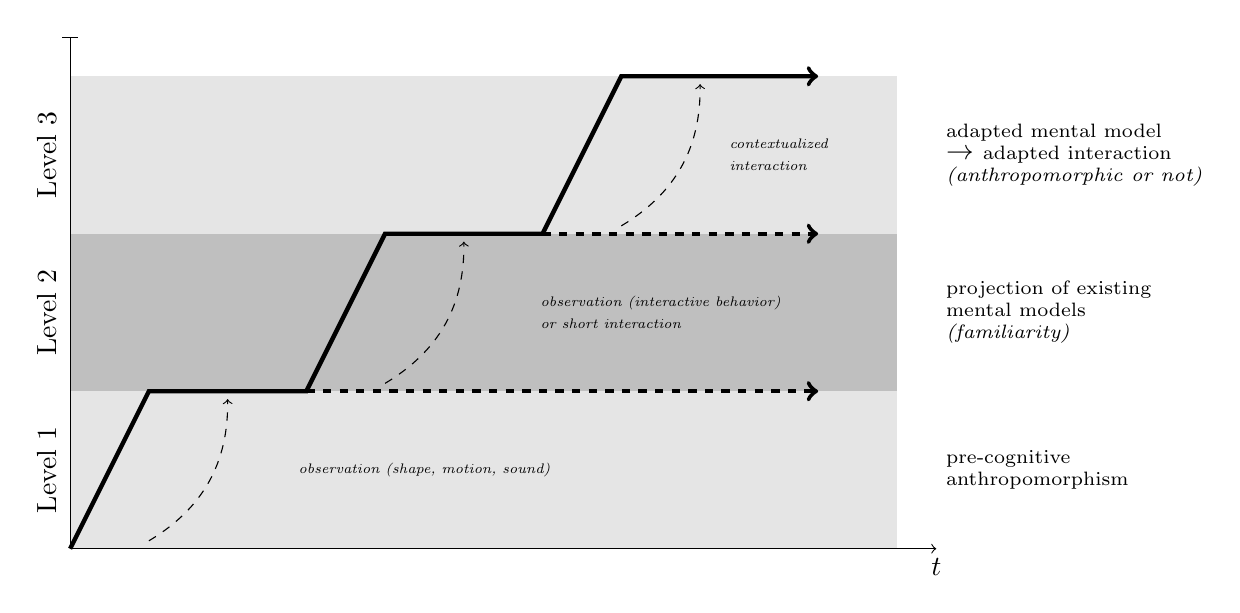
\begin{tikzpicture}
\baselineskip=8pt

\path[fill=gray!20] (0,0) rectangle (10.5,2);
\path[fill=gray!50] (0,2) rectangle (10.5,4);
\path[fill=gray!20] (0,4) rectangle (10.5,6);

\draw (-0.3,1) node[rotate=90] {Level 1}
      (-0.3,3) node[rotate=90] {Level 2}
      (-0.3,5) node[rotate=90] {Level 3};

\draw[->] (0,0) -- (11,0) node[anchor=north] {$t$};
\draw[-|] (0,0) -- (0,6.5) node[anchor=east] {};
% Us
\draw[ultra thick, ->] (0,0) -- (1,2) -- (3,2) -- (4,4) -- (6,4) -- (7,6) --
(9.5,6);
\draw[ultra thick, dashed, ->] (3,2) -- (9.5,2);
\draw[ultra thick, dashed, ->] (6,4) -- (9.5,4);

\draw (11,1) node[align=left, anchor=west]{\scriptsize pre-cognitive\\\scriptsize anthropomorphism}; %label

\draw (11,3) node[align=left, anchor=west] {\scriptsize{projection of existing}\\\scriptsize{mental models}\\\scriptsize{\it (familiarity)}}; %label

\draw (11,5) node[align=left, anchor=west] {\scriptsize{adapted mental
model} \\ $\to$ \scriptsize{adapted interaction}\\\scriptsize{\it (anthropomorphic or not)}}; %label


\draw[dashed,->] (1,0.1) to[bend right] (2,1.9)  node at (4.5,1) {\tiny{\it observation (shape, motion, sound)}}; %label

\draw[dashed,->] (4,2.1) to[bend right] (5,3.9)  node[align=left] at (7.5,3) {\tiny \it observation (interactive behavior) \\ \tiny \it or short interaction}; %label

\draw[dashed,->] (7,4.1) to[bend right] (8,5.9)  node[align=left] at (9,5)
{\tiny \it contextualized\\ \tiny \it interaction}; %label

\end{tikzpicture}
%}
\caption{The three cognitive levels of anthropomorphism: Level 1 is the instinctive,
sub-cognitive identification of living peers. {\it Empathy} is characteristic
of this stage. After longer observation or short, non-contextualized interaction
(typically, a lab environment), the user reaches Level 2: the user projects a
mental model he/she is already familiar with onto the robot. After longer {\it
contextualized} interaction (typically, at home), the user enters Level 3 of
anthropomorphism: the user recomposes an accurate mental model of the robot,
based on experience. This leads to adapted interaction modalities, that may
still be anthropomorphic, or not.}
\label{fig:cognitivemodel}
\end{figure}



We propose three different cognitive phases (Figure~\ref{fig:cognitivemodel}),
which do not directly match the previously presented three phases of
anthropomorphism but are still related.


\subsubsection{Cognitive Processes and Phases}

The main underlying cognitive process in anthropomorphism is understood as
perceiving and reasoning about something non-human and unfamiliar based on one's
representation of the familiar and well-known concept of being
human~\cite{epley_when_2008}. This led us to interpret the phases of
anthropomorphic interactions as parallel cognitive phases
(Figure~\ref{fig:cognitivemodel}).

The so-called \emph{level 1} is the instinctive, pre-cognitive identification of
living peers. That humans tend to anthropomorphize robots intuitively in this
pre-cognitive way
is supported by studies done by Rosenthal-von der Pütten
\textit{et al.}~\cite{rosenthal-vonderputten_experimental_2013} who investigated
the neural correlates of emotional reactions of humans towards a robot. {\it
Empathy} is characteristic of this stage~\cite{rosenthalvonderPutten2013neural}.
It is also at this stage that automatic activation of the human's mirror neurons
system  in response to viewing the robots action and human automatic emotional
responses are contributing at a lower level
to the intuitive anthropomorphization (see Section 2.2.2 \fixme{put ref})
%We suggest that the human's mirror neuron system is contributing to anthropomorphism by  allowing for a mapping of the robot's goal-directed actions into the human own motor repertoire \cite{Gallese1998, Wolpert2003, cullen2013individual}.


%mediated by the motor and emotional resonnance mechanisms at the neuronal level. 

After a longer observation period (typically including complete action sequences
of the robot) or short interaction (touching, short talk like greetings), we
suggest the human reaches the cognitive \emph{level 2}: in this phase, the human
starts building a behavioral and cognitive model of the robot that would support
both the observed and imagined capabilities of the robot.  The \emph{familiarity
thesis}~\cite{hegel_understanding_2008} supports the idea that the human
first projects onto the robot mental models of similar agents he/she is already
familiar with (ranging from animals to human adults, to pets and children). We 
hypothesize that the nature of the projected mental
model, as well as how deep the human engages in this projection, might be
driven by the same parameters as we mentioned for the \emph{initial capital of
anthropomorphism} (section~\ref{sec:ica}). 
At this stage the human might also change his attitude towards the robot, paying more attention to social cue than to low-level behaviour which may reinforce the resonnance mechanisms. 

The cognitive \emph{level 3} is reached after a \emph{contextualized} interaction.
A \emph{contextualized} interaction is \emph{explicitly purposeful} (the purpose
of the interaction, be it purely entertainment, is explicit and conscious to the
human), and takes place in an environment that fosters a stronger cognitive (and
possibly affective/social) commitment from the human in the interaction
(typically, at home). During this interaction, the human iteratively restates
and reshapes his/her behavioral and mental model of the robot (\emph{How does
the robot react to such and such situation/input?  What does the robot know
about me? About itself? About our environment? What can the robot learn?}, etc.).

This mental process depends on the human understanding of the robot's
inner working, as well as his/her own tendency to anthropomorphize (the
\emph{personality} in ICA factor), but at this
stage, the \emph{perception} of the robot (its shape for instance) and its
intended \emph{purpose} play a less important role. It is mostly a human-centric
process.  The result of this third phase would be an iteratively adapted
cognitive model of the robot. It is also at this last stage that the human might
modified its own abilities to anthropomorphize, having built a full cognitive
model of the robot and know being able to attribute internal state to the robot
through his theory of mind.


\subsection{Relation to the dynamics of anthropomorphism}

These cognitive levels overlap over time but do not exactly match the
\emph{Initialization}, \emph{Familiarization} and \emph{Stabilization} phases
introduced in our model of the dynamics of anthropomorphism. In particular,
the cognitive levels 1 and 2 are both included in the \emph{initialization} phase
of the anthropomorphism model. Sub-cognitive anthropomorphism typically
\emph{initiates} the novelty effect by rapidly engaging the human in the
interaction through an initial projected agency, whereas cognitive level 2
(projection of familiar mental models) supports the novelty effect by inducing
beliefs that the robot is set up with possibly complex cognitive abilities.

The cognitive level 3 also overlaps with the \emph{Familiarization} phase: as
the human gets used to the robot, we hypothesize one restates and adapts its
cognitive model of the robot by iteratively reshaping pre-existent, familiar
models until it provides a satisfying support to explain and justify the
observed robot behavior.

A \emph{stable level of anthropomorphism} is reached when the adaptation process
depicted in the cognitive level 3 reached a stable state, \ie the user's
experience with the robot is correctly supported by the cognitive model he/she
has built.

\subsection{Role of disruptive behaviors}
\label{sec:disruptive}

A cognitive interpretation of anthropomorphism also allows to better interpret
the role of unexpected robot behaviors, that we are \emph{disruptive} in regard
to the cognitive process of building a mental model of the robot.

Common observation of naive people (children or adults) interacting with robots
shows that unexpected behaviors of the robot can have a notable impact on
interaction. \hl{cite literature, e.g. cheating robot, disagreeing, disobeying,
HRI2013 paper}
This is supported by the results from \citet{Waitz2010} seen in section
\ref{sec:explanations} that people attribute more easily anthropomorphic
features to artefacts when they have unpredictable behaviors.

During a normal interaction with the robot, the user iteratively refines his/her
own model of the behavior of the robot. As explained in previous sections, as
the user improves his/her model of the robot's actions, he/she also improves the
ability to predict the actions and thus, the user tends to anthropomorphize
less.

We emit the hypothesis that an unexpected robot behavior might lead the user to
suddenly restate his/her behavioral model of the robot and will temporarily lead
to an increase of the level of anthropomorphism (depicted by the spikes on
Figure~\ref{fig:dynamics}).



\begin{figure}\footnotesize
    \centering
    \begin{tabular}{  >{\centering\arraybackslash}m{2cm} | >{\centering\arraybackslash}m{2cm} | >{\centering\arraybackslash}m{2cm} }
     & Unplanned by the robot & Planned by the robot \\ \hline
    Perceived as non-intentional & case I  & case IIIa  \\ \hline
    Perceived as intentional &  case IIIb & case II 
    \end{tabular}
\caption{
    Behaviors of the robot that are unexpected by the user may be intentional
    (the robot has planned the behavior) or not (typically, a failure:
    misdetection, bug,...). Independently of that, the behavior may be
    \emph{perceived} by the user as intentional or not.}
\label{fig:perceptionUnexpectedBehavior}
\end{figure}

When talking about \emph{unexpected robot behaviors}, several distinct cases
must however be considered, summarized in
Table~\ref{fig:perceptionUnexpectedBehavior}.

If the unexpected behavior is not planned, and perceived as such by the human
(case I), the human can interpret that the robot is able to fail. If the robot
explicitly states its failure (for instance, by saying ``I'm lost!''), the
behavior is then called \emph{transparent} \fixme{cite here, Julia?}
\hl{(literature on transparency)}, and the user may besides hypothesize that the
robot has \emph{introspective} capabilities (it can reflect on its own internal
state), which in turn may leads to higher anthropomorphism level.  On the
contrary, if the robot shows no sign of recognizing its own failure, the user
may ascribe a lower level of anthropomorphism to the robot.

In case II, the robot voluntary executes a behavior that is unexpected by the
human, and the human perceives it rightfully as an \emph{intentional} behavior.
For instance, the human asks the robot to go somewhere, and the robot refuses,
saying ``I do not want to go there''. In that case, we expect to see an increase
of anthropomorphism attribution due to the human ascribing intentionality to the
robot.

Case IIIa and IIIb correspond to misinterpretations of the robot behavior. Case
IIIb may actually lead to an increased level of anthropomorphism since the human
will (wrongfully) attribute intentionality to the robot, while case IIIa is
expected to lead to a lower anthropomorphism level.  However, in those two
cases, the next occurrence of an expected behavior, if correctly interpreted
(case I or II), is likely to lead to stronger effects due to a larger delta
between expectations and actual observed behavior. \hl{(we actually assume that
anthropomorphism can be radically changing and be a very spontaneous
"reaction".)}

%% experience -> unexpected behavior should not impact the interaction child-robot BEFORE the theory of mind is established!


%%%%%%%%%%%%%%%%%%%%%%%%%%%%%%%%%%%%%%%%%%%%%%%%%%%%%%%%%%%%%%%%%%%%%%%%%
%
%
%
%				DISCUSSION + FUTURE WORK
%
%
%
%%%%%%%%%%%%%%%%%%%%%%%%%%%%%%%%%%%%%%%%%%%%%%%%%%%%%%%%%%%%%%%%%%%%%%%%%

% JULIA & SEVERIN: how to measure / quantify anthropomorphism ...
% CLAIRE: FMRI study idea

\section{Discussion}
\label{sec:discussion}

The model of anthropomorphism we propose is still a work in progress. In
particular, its implications regarding the design of (social) robots and
human-robot interaction are still to be refined.

\subsection{Effect of Time and Familiarization}

\fixme{Discuss here the general findings of the paper: the global shape of the
model of the dynamics, ...}

The \textit{context of use} is related to the purpose (and functionality) of the
robot and influences the user interaction experience. With \textit{time}, we
refer to long-term interaction with the robot, which is related to what has been
described as \textit{novelty effect} but also accounts for the user getting used
to the robot. Consequently, we propose that anthropomorphism is not static but
likely to change, due to what we call \textit{dynamics}, in space and time.


As outlined in section \hl{XX}, the tendency to anthropomorphize is motivated by
a person's wish to make sense of an agent which might be difficult to understand
(in its functionality or behavior, for instance). In turn, a user might ascribe
intentions or emotions to the system because the systems output was unexpected
for the user. Based on this explanation, we estimate that when the user has
familiarized herself / himself with the system, thus reached the point of when
the system is usable and explainable, the tendency to anthropomorphize
decreases. Therefore, our second hypothesis is as follows: 

\begin{itemize}
    \item \textbf{Hypothesis 1} A person's tendency to anthropomorphize a robot
        is impacted by the context of use and purpose of the robot. A social
        context and purpose of the robot increases anthropomorphism.
        \textit{(context and purpose of the robot)}
	\item \textbf{Hypothesis 2} A person's tendency to anthropomorphize a robot decreases over time and with growing experience the person has with the robot. \textit{(familiarize oneself with the robot)}
\end{itemize}


Given our first hypothesis from above, this might not hold over all contexts;
more concretely, probably not in a social context of usage.


Smart innovative devices, such as personal domestic robots, might demand from a
human user spontaneous usage of an unfamiliar system. Such situations will
require that a user should be able to build up a mental model quickly, which
particularly holds for novice users \cite{schmitz_concepts_2011}.

Eddy \textit{et al.} points out that familiarity increases the tendency to
anthropomorphize \cite{eddy_attribution_1993}.

"As shown in several psychological experiments [13,24] and pointed out by Watt
[25], familiarity may also ease social acceptance and even tend to increase
people's tendency to anthropomorphize [16]." \cite{duffy_anthropomorphism_2003}


\subsection{Limitations}

The model of anthropomorphism we propose is still a work in progress. In
particular, its implications regarding the design of (social) robots and
human-robot interaction are still to be refined.

\subsection{General observations}

By adopting both a cognitive and a dynamic perspective on the anthropomorphic
bonds that establish between a robot and a human during an interaction, some
observations can be raised.

For instance, we propose that the human \emph{adapts} iteratively to the robot
by restating its cognitive model of the robot. Could our two models be
conversely relied on to have the robot itself iteratively adapting its
behavior? In particular, we hypothesize that the so-called novelty effect
represents a peak in anthropomorphic manifestations, followed by mostly
deception-driven refinements of the cognitive behavioral model of the robot.
Could we imagine that the robot pro-actively \emph{verbalizes} its own limits,
in a timely manner (likely before the end of the novelty effect). And how would
this affect the cognitive models built by the human?

One related question we plan to elaborate on is the effects of \emph{mutual
explicitation of the mental model of the other agent}: a human and a robot
interact on a given task, and after a while, we interrupt the task and ask each
of the agents to explicit the mental model it has built of its partner
(emotional state, beliefs, intentions, etc.). Depending on the cognitive levels
the two agents are in, we may expect varying accuracy levels in the produced
mental models.

Another question raised by these models relates to their transposition to
human-human interaction: while concepts like \emph{novelty effect} are not
directly meaningful when analyzing human-human interaction, insights from
cognitive sciences (and in particular social psychology) regarding how we, as
humans, cope with unexpected behaviors from peers, or on the dynamics of mental
model refinements, could bring interesting perspectives with possible
applications to better manage long-term human-robot interactions.

\subsection{Measuring anthropomorphism}
\label{sec:measuring}

\fxwarning{To be completed/rephrased into a discussion}

\citep{ruijten_introducing_2014}

Also, the methods and measurements applied to study anthropomorphism appear insufficient, when applying a holistic understanding of anthropomorphism emerging from an interaction between a human user and a robot, for instance. Our point here is that to study a phenomenon as complex as anthropomorphism, we believe that one needs to take into account many factors (see Section \ref{sec:multi-factors}), besides looking at the human-like design of the artifact.
However, most of the
experiments that investigate anthropomorphism in robotics are conducted in
controlled lab-settings during short-term human-robot interactions. This
experimental setting can be critical for studying
anthropomorphism and findings might possibly lead to interpretations that would not be generalizable to natural settings or real interaction scenarios. For instance, some studies are about showing pictures of different robots to human subjects and then asking them how "human-like" they would rate these robots. What points of reference do the participants have in this setting? What can you really tell from a picture? I found that some normal people totally misinterpret the size / height of a robot, when it is not indicated. Also, when showing only pictures, movements, behaviors, materials, and so forth are totally disregarded. However, these aspects are also crucial to assess how "human-like" a robot appears. Last but not least, it has been found that "human-likeness" is a quite diverse and abstract term that includes many things. Instead of asking such a big question, \cite{kahn_jr._robotic_2006} suggest to ask for more concrete constructs that are typical or unique of the concept of "human-likeness", such as being hungry or feeling guilty. For instance, \cite{ruijten_introducing_2014} propose a 25 concrete questions to measure anthropomorphism along a scale that accounts for lower and higher levels of it.
Some studies (e.g. exploring characteristics of the "uncanny valley") also seem to contrast two or
more different anthropomorphic or mechanical systems that might not be
appropriate for comparison given the complex context. 


Measuring anthropomorphism is challenging because the phenomenon is partially
unconscious, its mediation is largely subject-dependent\fxnote{Should we put
here different interaction profiles from the Ranger study?}, and we found the
phenomenon generally difficult to verbalize for users.

To reduce subjectivity and still accurately account for psychological effects,
it appears necessary to interleave quantitative and qualitative assessments of
anthropomorphic effects.

We present in this section the methodology and techniques we have relied on to
assess anthropomorphic projections in two unrelated studies, the Roomba
experiment~\cite{fink_living_2013}, and the Domino study.

\paragraph{Quantitative assessment of anthropomorphism} Quantitative data are
acquired by systematic annotations of human- robot interactions on video records
of the experiments. Six classes of interactions were identified as reflecting
active commitment of the users in the interaction (gestures, touches, talk to
the robot, show something to the robot, misbehave, look at the experimenter
because worried by the robot's behavior)

\paragraph{Qualitative assessment of anthropomorphism} The main tools for
qualitative measurement of anthropomorphic effect are questionnaires. We have
explored both Likert-scale and open questions. In the Domino study,
questionnaires were analyzed such as points are attributed for key answers,
leading to a qualitative score:

\begin{itemize}
    \item Spontaneously ascribe feelings or states (2 points) {\it Robot is
        hungry, tired}
    \item Ascribe ``own will'' (1--3 points) {\it Robot could leave room, does not
        always obey, could do a b\^{e}tise...}
    \item View robot as friend (1 point)
    \item Ascribe cognitive abilities (0.5--1 point) {\it Robot is able to see,
        able to hear}
    \item Belief robot has feelings (2 points)
    \item Give anthropomorphic reasons for
        \begin{itemize}
            \item not leaving robot alone (1--3 points) {\it Would be sad when
                left alone}
            \item misbehavior (1 point) {\it Robot wants to make a tour, doesn't
                like to play any longer}
        \end{itemize}
\end{itemize}

\subsection{Sustaining long-term interaction}

\paragraph{Impact of the behavioral complexity of robots}

To remain tractable, most experiments, and even more when they investigate
long-term interactions, are carried with robots exhibiting relatively simple
behaviors. In our model, the maximum level of anthropomorphism \AntMax is
reached at the end of the novelty effect, and then decrease. A natural question
is whether we can design robots such as \AntMax remains high, possibly higher
than $\ant[t_{novelty~peak}]$ (note that to know if sustaining strong
anthropomorphic interaction is desirable is entirely another question).

Intuitively, the behavioral complexity of the robot, and in particular, the ability
for the robot to evolve over time and adapt its behavior to the user as the user
familiarizes itself with the robot (\ie, \emph{co-familiarize}), seems to play a
key role.

...

\subsection{Ethical aspects of anthropomorphism and human-like form of robots}

% our message kind of is that it would be favorable to sustain anthropomorphism over 
% extended periods of time ... however, this is ethically questionable, when thinking 
% of emotional bonding with an artificial agent, etc. --> we sould elaborate on this a % bit

Another critical point with the use of human-like form in artificial agents are 
ethical aspects. For instance, we need to consider how far we actually want an 
\textit{artificial agent} to resemble a human -- or ourself. Even though we do not 
discuss these aspects in this article, we think the HRI / robotics community needs 
to consider questions of how far an artificial agent should act ``as if it would be 
social'' toward humans. What implications does an anthropomorphic design of robots 
have? What happens as soon as the artificial agent is considered a \textit{moral 
agent} \cite{sullins_when_2006}? Using \textit{socially interactive robots} in 
contexts involving elderly care or rehabilitation for disabled / handicapped 
persons, autistic children is a controversially discussed topic 
\cite{robins_robots_2005}.


%%%%%%%%%%%%%%%%%%%%%%%%%%%%%%%%%%%%%%%%%%%%%%%%%%%%%%%%%%%%%%%%%%%%%%%%%
%
%
%
%				CONCLUSIONS
%
%
%
%%%%%%%%%%%%%%%%%%%%%%%%%%%%%%%%%%%%%%%%%%%%%%%%%%%%%%%%%%%%%%%%%%%%%%%%%

% JULIA & SEVERIN

\section{Conclusion}
\label{sec:conclusion}

Our data suggest that there are qualitative differences and dynamics over time
in how humans relate to different types of robots. More concretely, we found
that people's perception of human-likeness in the robot and in turn their
human-social engagement with the robot was not only based on how much the robot
resembled a human (mostly in its behavioral cues) but that this was determined
by multiple factors, including individual characteristics of the human user but
also the context of use, for instance. Interestingly, our findings also suggest
that how far people anthropomorphize a robot is likely to change over time with
growing experience of the user with the system. 

Based on these observations and an extensive literature review, we would like to
propose a model that accounts for variances and dynamics in anthropomorphism.
This model of the \textit{``Dynamics of Anthropomorphism''} considers several
impact factors, including the human user, the anthropomorphic design of the
non-human agent, the context of use, and the interaction experience (time). With
this initial model, we would like to extend the current understanding of
anthropomorphism in robotics and human-robot interaction. This might in turn
lead to a discussion about the short- and long-term benefits and other effects
of the human-like (anthropomorphic) design of robots and other artificial
agents.


Anthropomorphism is a social phenomenon which seems to be natural on one side
and very complex on the other side. It is a mechanism within oneself that makes
a human observer think and treat a non-human agent as if it would have some
human (social) characteristics, and ascribe to it intentions, emotions, or
thoughts, for instance. Understanding the reasons and modalities of
anthropomorphism is thus of prime importance to build a successful and lasting
human-robot interaction.

While anthropomorphism is traditionally empirically understood as the
interactions between the anthropomorphic design of a robot and the psychological
determinants of the user, it appears that the duration and context of the
interaction are also key factors, and that anthropomorphism needs to be
understood as a dynamic phenomenon. In this article, we propose a new formal
model of anthropomorphism that accounts for these three factors and also
explicits the dynamics of anthropomorphism. We introduce the concepts of
\emph{initial} and \emph{stabilized levels of anthropomorphism} as compound
factors to characterize the profile of a given anthropomorphic interaction.

The article also discusses the cognitive correlates of anthropomorphism. We
proposes to identify three cognitive levels corresponding to successive
refinements of the mental models of the robot that the user builds during the
interaction. We show how these levels relate to observable anthropomorphic
effects, and how they evolve over time.

While subject to discussion and further extensions, we hope that this
contribution consolidates the scientific grounds of anthropomorphism, and
provides support for a better understanding of long-term acceptance of robots in
human environments.


\section*{Acknowledgments}

This research was supported by the Swiss National Science Foundation through the National Centre of Competence in Research Robotics.

%\section{Bibliography}

\bibliographystyle{frontiersinSCNS&ENG} % for Science and Engineering articles
\bibliography{dynamics-anthropomorphism}   % name your BibTeX data base


\end{document}
